\documentclass[runningheads]{llncs}

\usepackage[T1]{fontenc}
\usepackage{graphicx}
\usepackage{amsmath}
\usepackage{amssymb}
\usepackage{booktabs}
\usepackage[table]{xcolor}
\usepackage{array}
\usepackage{multirow}
\usepackage{float}
\usepackage{placeins}
\raggedbottom
\setlength{\textfloatsep}{10pt plus 2pt minus 4pt}
\setlength{\floatsep}{8pt plus 2pt minus 2pt}
\setlength{\intextsep}{8pt plus 2pt minus 2pt}

\newcommand{\best}[1]{\cellcolor{gray!55}\textbf{#1}\textsuperscript{*}}
\newcommand{\second}[1]{\cellcolor{gray!33}\textbf{#1}}
\newcommand{\third}[1]{\cellcolor{gray!16}#1}
\newcommand{\OpenAlex}{\mbox{OpenAlex}}

\begin{document}

\title{Learning Adaptive Graphs to Uncover Potential Relationships for Scientific Topic Popularity Trend Forecasting}
\titlerunning{AG-FC for Multivariate Topic Popularity Forecasting}

\author{Changwang Li\inst{1,2} \and Xuecan Tian\inst{1,2} \and Zeyu Deng\inst{1,2} \and Jin Mao\inst{1,2}\thanks{Corresponding author: \texttt{maojin@whu.edu.cn}.}}
\authorrunning{C. Li et al.}

\institute{Center for the Studies of Information Resources, Wuhan University, Wuhan 430072, China \and
School of Information Management, Wuhan University, Wuhan 430072, China}

\maketitle

\begin{abstract}
Forecasting scientific topic popularity from historical bibliometric signals is important for hotspot monitoring, strategic research planning, and evidence-informed science policy. We formulate this problem as multivariate annual publication-volume forecasting across correlated topics or subfields, where the main challenges are coupled cross-topic dynamics and incompletely observed relations. To address these issues, we propose AG-FC, an adaptive graph forecasting framework built on the Fully Connected Gated Graph Architecture (FC-GAGA) backbone. AG-FC replaces the original graph gate with adaptive topology learning and further introduces SVD-initialized adaptive or hybrid modes to combine latent dependencies with co-occurrence priors. Experiments on eight \OpenAlex subsets (four domains and four computer-science subfields) demonstrate that AG-FC is highly competitive overall, outperforming baselines in 12 out of 24 evaluation metrics. Notably, it achieves substantial gains at the finer subfield level (winning 11 of 12 metrics) while maintaining competitive domain-level performance. Compared with FC-GAGA and its graph-gate-removed variant, AG-FC improves upon 20 and 21 out of 24 evaluation settings, respectively. Finally, while the adaptive-only mode maximizes raw numerical accuracy, the SVD-enhanced hybrid mode preserves structural priors for interpretable scientometric analysis while remaining highly competitive in forecasting performance.

\keywords{scientific topic popularity forecasting \and multivariate time-series forecasting \and adaptive graph learning \and potential relation discovery}
\end{abstract}

\section{Introduction}
Forecasting scientific topic popularity is important for hotspot monitoring, strategic research planning, and evidence-informed policy. We define topic popularity as annual publication volume and formulate the task as multivariate forecasting: given historical annual publication series of multiple related topics or subfields, jointly predict their future publication counts.

Compared with independent univariate extrapolation, this setting introduces three key challenges: \textbf{(C1) coupled temporal dynamics} across topics, \textbf{(C2) incomplete observed relations} in predefined co-occurrence graphs, and \textbf{(C3) uncertainty in how to optimally combine prior topology with adaptively learned dependencies}.

To address these issues, we propose AG-FC (Adaptive Graph Fully Connected), built on the FC-GAGA architecture with an N-BEATS residual forecasting backbone \cite{Oreshkin2020N-BEATS:,oreshkin2021fc}. AG-FC replaces the original graph gate with adaptive topology learning \cite{wu2019graph} and introduces an SVD-enhanced hybrid fusion mode to balance latent relation discovery with prior consistency.
Given the low-frequency annual setting and limited effective sample size, the backbone should separate smooth long-term drift from bursty perturbations while remaining stable under short histories. In publication-volume series, yearly trajectories typically mix smooth disciplinary drift with burst-like fluctuations triggered by methods, events, or policy shifts. FC-GAGA is a pragmatic temporal base because it inherits N-BEATS residual decomposition: iterative residual correction separates low-frequency trend components from higher-frequency variation without relying on heavy recurrence. Prior evidence in long-span macroeconomic forecasting also shows that N-BEATS-style residual subtraction remains effective when temporal samples are limited, where heavier Transformer alternatives are not consistently superior \cite{wang2022ecoforecast}. We therefore use FC-GAGA as a robust temporal backbone rather than as a claim of universal optimality; its original graph gate, however, remains relatively naive and prior-dependent, motivating our adaptive topology and fusion design.

Our core contributions are:
\begin{enumerate}
    \item We reformulate topic popularity forecasting as topology-aware multivariate prediction over correlated topic and subfield series.
    \item We introduce adaptive graph learning to uncover latent cross-topic dependencies and improve forecasting performance.
    \item We design an SVD-enhanced hybrid topology mode that provides a practical trade-off between predictive accuracy and prior-consistent relation analysis.
\end{enumerate}

Experiments on eight \OpenAlex{} subsets reveal a clear granularity pattern. AG-FC is strongly competitive overall, securing top-1 results in 12 out of 24 evaluation metrics, with particularly substantial gains at the finer subfield level (winning 11 of 12 metrics). Relative to FC-GAGA and its graph-gate-removed variant, AG-FC outperforms them in 20 and 21 out of 24 evaluation settings, respectively; data and code are available at \texttt{https://github.com/navfour/AGFC}.
Ultimately, these results support a central thesis of this work: latent relational structure is a first-class signal in topic forecasting and must be modeled jointly with temporal dynamics. More broadly, this motivates a graph-temporal scientometrics perspective in which forecasting and structure discovery are integrated rather than separated, providing more transparent evidence for research planning and funding decisions.

\section{Related Work}
\subsection{Topic Trend Forecasting in Scientometrics}
Scientific topic popularity trend forecasting is a central task in scientific intelligence and strategic planning because it supports forward-looking identification of emerging frontiers and informed allocation of research resources. The underlying challenge is that knowledge evolution is multivariate and dynamic, driven by both domain-internal logic and external social, technological, and economic factors. Compared with purely expert-driven judgment, computational forecasting from large-scale scholarly corpora is more scalable and reproducible.

Existing studies generally follow two perspectives. The first places emphasis on mining the evolutionary trends and evolution patterns of research topics, and on dynamically observing likely future directions to support forward-looking decision making and strategic planning. A typical pipeline extracts latent topics, tracks temporal changes in topic intensity (e.g., emergence, persistence, and decline), and then interprets or ranks topics according to evolution-related characteristics. Dynamic topic modeling and structural topic modeling are representative approaches in this line \cite{lou2023diversity,kraus2023moon}. However, these studies mainly provide evolutionary characterization and ranking, and objective out-of-sample forecasting accuracy is harder to evaluate consistently.

The second treats topic trend prediction as a time-series forecasting task, leveraging existing forecasting algorithms to more directly capture future trend trajectories from historical indicators. Under the shared label of topic trend prediction, studies may optimize different goals, including regression-style forecasting, emerging-topic identification or ranking, relation-aware forecasting, and descriptive trend analysis \cite{xu2022scientific,chen2018modeling,rahimi2023atem,liang2021combining,chi2022incorporating,zheng_research_2022}. Our work belongs to the regression-style multivariate forecasting perspective.

\subsection{Temporal Backbones for Multivariate Forecasting}
Under this paradigm, topic trends are typically quantified as temporal signals such as topic frequency, publication volume, citation impact, or composite popularity indicators \cite{xu2022scientific,chen2018modeling,wang2025knowledge,rahimi2023atem,liang2021combining}. Early studies mainly relied on statistical extrapolation such as ARIMA \cite{zou2024research,abuhay2018towards}. Later pipelines combined feature-based machine learning and neural forecasting. In deep forecasting, recurrent backbones such as RNN and LSTM improved nonlinear temporal modeling \cite{lu2019evolutionary,xu2022scientific}, while Transformer-style MTS models strengthened long-horizon modeling through efficient attention, decomposition, and tokenization-based mixing \cite{zhou2021informer,wu2021autoformer,nie2022time,zhang2023crossformer}. More recent mixers further improved temporal-variable interaction efficiency in multivariate settings \cite{wang2024timemixer,wang2024timexer}.

Despite these advances, most temporal backbones still operate on regular Euclidean tensors and learn cross-topic dependence implicitly. The common mechanism is tensor-level temporal-variable mixing on regular grids. This is effective for long-range sequence modeling, but relation modeling remains implicit because interactions are encoded as dense latent mixing patterns without explicit distinction between observed topology and unobserved dependencies. In scientometric systems with sparse, asymmetric, and time-varying relations, purely tensor-based coupling can underutilize structured prior information and miss weak but predictive latent links. Relation-aware pipelines based on precomputed features or sequence-level coupling can partially alleviate this issue \cite{chi2022incorporating,zheng_research_2022}, but topology remains external to the forecasting objective, so weak or higher-order links are easily lost.

Graph-temporal forecasting addresses this issue more directly by integrating temporal modeling and graph propagation \cite{li2021spatial,shao2022decoupled}. However, many topic-focused designs still rely on predefined static graphs and relatively weakly adaptive topology modules, making performance sensitive to prior-graph completeness. Because co-occurrence priors in scholarly data are often noisy, partial, and time-varying, forecasting models should jointly exploit observed relations and adaptively learn latent dependencies. This motivates the adaptive-graph focus in Section~2.3 and the method design in Section~3.

\subsection{Adaptive Graph and Topology Learning}
Adaptive graph learning directly addresses fixed-adjacency limitations. Graph WaveNet and AGCRN show that data-driven topology can recover latent dependencies beyond predefined graphs \cite{wu2019graph,bai2020adaptive}. Follow-up studies further explore dynamic graph construction and progressive adjacency updates \cite{li2023dynamic,duan2025dynamic}. Recent work also emphasizes scalability and robustness of adaptive graph design \cite{shin2024pgcn,ma2025less}.

For topic forecasting, the remaining gap is not only accuracy but also interpretability relative to prior scientometric structure. In our setting this leads to two coupled requirements: discover latent relations beyond co-occurrence priors, while preserving a controllable connection to prior topology for relation analysis. AG-FC maps these requirements to two design choices: adaptive topology learning for latent dependency discovery, and SVD-initialized hybrid fusion for prior-consistent yet flexible relation modeling, replacing the naive FC-GAGA graph component \cite{oreshkin2021fc}.

\section{Method}
\subsection{Problem Formulation}
We study \emph{topic trend popularity forecasting}, where the prediction target is future annual publication volume for a set of related scientific entities. Depending on the dataset level, each node denotes either a subfield (domain-level datasets) or a topic (subfield-level datasets), and each node has an annual publication-count series.

This task is converted into a graph-aware multivariate time-series forecasting problem. The temporal dependency comes from yearly publication trajectories, while the relational dependency comes from inter-node topology (e.g., co-occurrence-based prior graph). We use $T$ to denote the historical look-back length and $H$ to denote the forecasting horizon. In the experiments reported in this paper, we use a one-step-ahead setting ($H=1$, i.e., only $h=1$ is evaluated), which aligns with annual strategic planning cycles in research management and policy contexts. The goal is to jointly forecast the next $H$ years for all nodes, rather than forecasting each series independently.

Formally, let $\mathbf{G}=(\mathbf{V},\mathbf{E})$ denote a prior topic graph. In general, such a graph can come from citation, co-occurrence, or semantic relations; in this study, all experiments use the co-occurrence graph constructed from OpenAlex multi-label assignments. Let $|\mathbf{V}|=N$ be the number of nodes, and let $\mathbf{A}\in\mathbb{R}^{N\times N}$ be its adjacency matrix, where $\mathbf{A}_{ij}=1$ if $(v_i,v_j)\in\mathbf{E}$ and $\mathbf{A}_{ij}=0$ otherwise.

Let $\mathbf{Y}_{1:T}=\{\mathbf{Y}_1,\mathbf{Y}_2,\ldots,\mathbf{Y}_T\}$ be the historical multivariate topic series, where $\mathbf{Y}_t\in\mathbb{R}^{N}$ is the observation vector at time step $t\in\{1,\ldots,T\}$. For node $n$, $y_{n,t}$ denotes its scalar value at time $t$ (e.g., publication count).

Given $\mathbf{G}$ and historical observations $\mathbf{Y}_{1:T}$, we learn a forecasting function $f_{\Theta}(\cdot)$ to predict the next $H$ steps:
\begin{equation}
\hat{\mathbf{Y}}_{T+1:T+H} = f_\Theta\bigl(\mathbf{Y}_{1:T},\mathbf{G}\bigr).
\end{equation}

For evaluation, let $T_{\text{test}}$ denote the test-set length (number of test timestamps), and let $y^{\text{test}}_{n,t}$ and $\hat{y}^{\text{test}}_{n,t}$ denote ground truth and prediction for node $n$ at test timestamp $t$ ($t=1,\ldots,T_{\text{test}}$). We report Mean Absolute Error (MAE), Mean Absolute Percentage Error (MAPE), and Root Mean Squared Error (RMSE):
\begin{equation}
\mathrm{MAE} = \frac{1}{N T_{\text{test}}}\sum_{n=1}^{N}\sum_{t=1}^{T_{\text{test}}}\left|y^{\text{test}}_{n,t}-\hat{y}^{\text{test}}_{n,t}\right|,
\end{equation}
\begin{equation}
\mathrm{MAPE} = \frac{100}{N T_{\text{test}}}\sum_{n=1}^{N}\sum_{t=1}^{T_{\text{test}}}\left|\frac{y^{\text{test}}_{n,t}-\hat{y}^{\text{test}}_{n,t}}{y^{\text{test}}_{n,t}}\right|,
\end{equation}
\begin{equation}
\mathrm{RMSE} = \sqrt{\frac{1}{N T_{\text{test}}}\sum_{n=1}^{N}\sum_{t=1}^{T_{\text{test}}}\left(y^{\text{test}}_{n,t}-\hat{y}^{\text{test}}_{n,t}\right)^2}.
\end{equation}
The RMSE above is a \emph{global RMSE} (single square root after aggregation over all node-time pairs), rather than averaging node-wise RMSE values.

\subsection{Overall Framework}
As shown in Fig.~\ref{fig:framework}, AG-FC follows the core FC-GAGA forecasting logic \cite{oreshkin2021fc}: an N-BEATS-style residual fully connected stack iteratively decomposes input history into backcast and forecast components. For residual block $r$, the input is updated by
\begin{equation}
Z_r=\operatorname{ReLU}(Z_{r-1}-Z^b_{r-1}),
\end{equation}
and each block outputs a backcast--forecast pair. Forecast terms are accumulated across blocks and then aggregated across stacks to produce the final prediction.

The key modification relative to FC-GAGA is the topology pathway. Instead of using a fixed and relatively naive graph gate, AG-FC introduces an adaptive topology module: it learns latent adjacency from node embeddings (Sec.~3.3), supports SVD-guided initialization and prior-aware hybrid fusion with co-occurrence graphs (Sec.~3.4), and propagates relational signals through $\phi_{\text{graph}}$ (GraphSAGE, GAT, or GCN). The resulting graph-aware representation is injected into the residual FC forecasting stream, so temporal decomposition and relational modeling are optimized jointly.
The execution order in each stack is: (i) construct or select adjacency, (ii) apply $\phi_{\text{graph}}$ on node features, and (iii) feed the graph-aggregated output directly into the FC residual blocks. There is no extra standalone FC projection module between $\phi_{\text{graph}}$ and the residual blocks (except the internal linear transforms that belong to the selected graph operator itself, e.g., GraphSAGE, GCN, or GAT).

\begin{figure}[htbp]
    \centering
    \begingroup
    \pdfimageresolution=300
    \includegraphics[width=\linewidth]{figs/model5.png}
    \endgroup
    \caption{\textbf{Left}: AG-FC forecasting cell with adaptive topology module, residual FC blocks, and stack aggregation. \textbf{Right}: graph-gather module that fuses a prior graph with adaptively learned adjacency from SVD-initialized node embeddings and graph convolution layers.}
    \label{fig:framework}
\end{figure}

\subsection{Adaptive Graph Learning}
To capture latent cross-topic dependencies beyond predefined edges, AG-FC learns an adaptive adjacency matrix directly from trainable node embeddings. Let $\mathbf{E}_1\in\mathbb{R}^{N\times d}$ and $\mathbf{E}_2\in\mathbb{R}^{d\times N}$ be learnable node-embedding parameters. We first compute a pairwise relation score matrix:
\begin{equation}
\mathbf{S}=\mathbf{E}_1\mathbf{E}_2,
\end{equation}
and then transform it into a nonnegative row-stochastic adaptive topology:
\begin{equation}
\mathbf{A}_{\text{adapt}}=\operatorname{softmax}\bigl(\operatorname{ReLU}(\mathbf{S})\bigr).
\end{equation}
The ReLU operation removes negative affinities, and row-wise softmax normalizes each node's outgoing weights into a probability-like distribution, yielding a directed adaptive graph. This adaptive topology is the core implementation of contribution 2, because it allows the model to discover latent relations that are not explicitly observed in the prior co-occurrence graph.

In the adaptive-only mode, graph propagation is performed directly on $\mathbf{A}_{\text{adapt}}$:
\begin{equation}
\mathbf{G}_{\text{adapt}}=\phi_{\text{graph}}(\mathbf{A}_{\text{adapt}},\mathbf{X}),
\end{equation}
where $\phi_{\text{graph}}(\cdot)$ denotes a graph aggregation operator that can be instantiated as GraphSAGE, GAT, or GCN. The model also supports a random-initialization branch for $\mathbf{E}_1,\mathbf{E}_2$, which corresponds to a naive Graph WaveNet-style adaptive graph setup.
The resulting $\mathbf{G}_{\text{adapt}}$ is then used as the direct input feature tensor of the FC residual stack.

Empirically, introducing this graph aggregation stage yields clear gains over the ``without graph gate'' variant, and GraphSAGE is the strongest and most stable choice in our setting. A plausible reason is that mean-based neighborhood aggregation is more robust to noisy and uneven co-occurrence edges, while avoiding the higher variance of attention-based weighting and excessive smoothing on sparse annual scholarly graphs.

\subsection{SVD-Enhanced Hybrid Topology Fusion}
Although adaptive-only learning can be strong in raw accuracy, a purely random-initialized adaptive graph may drift away from established prior knowledge, making discovered relations harder to align with domain understanding in practical use. In many settings, users prefer relation updates anchored to known structure, i.e., selectively amplifying or suppressing existing prior links instead of learning topology entirely from scratch.

Motivated by this requirement, we design a flexible topology module that supports multiple operating modes: adaptive-only (random or SVD-initialized), base-graph-only, and hybrid fusion. This design improves practical usability by allowing different trade-offs between predictive performance and prior consistency in relation analysis.

Let $\mathcal{P}_{\tau}$ be the set of papers in year $\tau$, and let $\mathcal{S}(p)$ denote OpenAlex labels assigned to paper $p$ (topic labels for subfield-level datasets and subfield labels for domain-level datasets). We construct the yearly co-occurrence matrix as:
\begin{equation}
\left[\mathbf{A}_{\tau}\right]_{ij}
=
\sum_{p\in\mathcal{P}_{\tau}}
\mathbb{I}\!\bigl(i\in\mathcal{S}(p)\ \wedge\ j\in\mathcal{S}(p)\bigr),
\quad i\neq j.
\end{equation}
For a sample at time $t$ with window length $L$, the window-level base graph is defined by temporal averaging:
\begin{equation}
\mathbf{A}^{(t)}_{\text{base}} = \frac{1}{L}\sum_{\tau=t-L+1}^{t}\mathbf{A}_{\tau}.
\end{equation}

To inject low-rank structural priors into adaptive learning, node embeddings are initialized by truncated SVD of the training base graph:
\begin{equation}
\bar{\mathbf{A}}_{\text{train}} \approx \mathbf{U}_{r}\mathbf{\Sigma}_{r}\mathbf{V}_{r}^{\top},\quad
\mathbf{E}_{1}^{(0)}=\mathbf{U}_{r}\mathbf{\Sigma}_{r}^{1/2},\quad
\mathbf{E}_{2}^{(0)}=\mathbf{\Sigma}_{r}^{1/2}\mathbf{V}_{r}^{\top}.
\end{equation}
Random initialization is also supported for comparison with the naive adaptive-graph setting.

Given $\mathbf{A}^{(t)}_{\text{base}}$ and $\mathbf{A}_{\text{adapt}}$, hybrid topology is formed through node-wise fusion:
\begin{equation}
\mathbf{m}=\exp(\mathbf{w}),\qquad
\mathbf{A}^{(t)}_{\text{hyb}}=
\operatorname{RowNorm}\!\left(
\mathbf{A}^{(t)}_{\text{base}}+
\operatorname{diag}(\mathbf{m})\,\mathbf{A}_{\text{adapt}}+\mathbf{I}
\right),
\end{equation}
where $\mathbf{m}$ is a learnable node-wise fusion strength vector.

For inference and training under different operating modes, the selected topology is:
\begin{equation}
\mathbf{A}^{(t)}_{\text{sel}} =
\begin{cases}
\mathbf{A}^{(t)}_{\text{base}}, & \text{base-only},\\
\mathbf{A}_{\text{adapt}}, & \text{adaptive-only},\\
\mathbf{A}^{(t)}_{\text{hyb}}, & \text{hybrid}.
\end{cases}
\end{equation}
The graph aggregation operator $\phi_{\text{graph}}$ (GraphSAGE, GAT, or GCN) then propagates block input $\mathbf{X}$ on $\mathbf{A}^{(t)}_{\text{sel}}$:
\begin{equation}
\mathbf{G}=\phi_{\text{graph}}(\mathbf{A}^{(t)}_{\text{sel}},\mathbf{X}).
\end{equation}
The resulting graph-aware features are fed into the FC residual forecasting stacks, allowing observed co-occurrence structure and latent dependencies to jointly shape predictions.

\section{Dataset and Exploratory Analysis}
Our datasets are built from OpenAlex \cite{priem2022openalex}, using its four-level hierarchical taxonomy (domain, field, subfield, and topic). We construct annual topic-level publication series for eight benchmark subsets across two granularity levels. At the domain level, we include all four OpenAlex domains for complete coverage: \texttt{domain 1} (Life Sciences), \texttt{domain 2} (Social Sciences), \texttt{domain 3} (Physical Sciences), and \texttt{domain 4} (Health Sciences). At the subfield level, we select four representative computer-science subfields with sufficient topic counts for stable multivariate forecasting: \texttt{subfield 1702} (Artificial Intelligence), \texttt{subfield 1705} (Computer Networks and Communications), \texttt{subfield 1707} (Computer Vision and Pattern Recognition), and \texttt{subfield 1710} (Information Systems). All subsets use a unified chronological split: 1975--2014 for training, 2015--2019 for validation, and 2020--2024 for testing. Data summaries and the node-level catalog are provided in Table~\ref{tab:dataset-summary} (Appendix~\ref{sec:appendix-exploratory}) and the supplementary material.

Exploratory diagnostics (Appendix~\ref{sec:appendix-exploratory}) show a clear granularity contrast. Domain-level graphs are dense and stable (density 73.92\%--84.24\%, turnover 8.66\%--11.47\%), whereas subfield-level graphs are sparser and more dynamic (density 14.87\%--49.31\%, turnover 28.56\%--45.58\%), with faster hotspot evolution and stronger structural change, especially in \texttt{subfield 1702}. Dynamic Time Warping (DTW) analysis further indicates meaningful lagged dependencies among topics or subfields. Together, these structural dynamics and cross-topic correlations motivate graph-temporal modeling over independent univariate forecasting.

\section{Experiment and Ablation Results}

\subsection{Overall Comparison Across Baselines}
Table~\ref{tab:table5} reports the main comparison against external baselines using our best-performing AG-FC setting (\texttt{adaptive only, without SVD}), while Table~\ref{tab:table5-ablation-split} details AG-FC mode ablations. For clarity, Table~\ref{tab:table5} highlights top-1 results only, whereas Tables~\ref{tab:table5-ablation-split} and~\ref{tab:graph-operator-summary} retain top-3 highlighting to show relative robustness.

We evaluate six complementary baselines that cover classical statistical, recurrent, and modern Transformer and mixer forecasting families: \textbf{SARIMAX} (classical linear trend extrapolation), \textbf{LSTM} (canonical nonlinear recurrent forecasting), \textbf{NeuralProphet} (modern neural trend-seasonality modeling), \textbf{Informer} (efficient Transformer forecasting), \textbf{TimeX++} (recent multivariate temporal mixing), and \textbf{FC-GAGA} (our direct predecessor, isolating the impact of adaptive topology replacement). We also include \texttt{FC-GAGA (without graph gate)} as a diagnostic variant.

\begin{table}[htbp]
\caption[Main-experiment comparison across external baselines and the best AG-FC setting.]{Main-experiment comparison across external baselines and the best AG-FC setting. AG-FC achieves the strongest overall performance, with particularly consistent gains on dynamic subfield-level datasets.}
\label{tab:table5}
\centering
\begingroup
\tiny
\setlength{\tabcolsep}{2pt}
\renewcommand{\arraystretch}{1.08}
\resizebox{\textwidth}{!}{%
\begin{tabular}{>{\centering\arraybackslash}m{2.7cm}c*{8}{c}c}
\toprule
Model or Setting & Metric & domain 1 & domain 2 & domain 3 & domain 4 & subfield 1702 & subfield 1705 & subfield 1707 & subfield 1710 & Top-1 \\
\midrule
\multirow{3}{*}{LSTM} & MAE & 2780.03 & 12757.84 & 4722.16 & 3987.47 & 1200.52 & 1039.94 & 1994.09 & 1479.49 & 0 \\
 & RMSE & 4907.51 & 23100.92 & \best{7792.88} & 8384.94 & 2675.26 & 1556.19 & 6499.11 & 4444.72 & 1 \\
 & MAPE & 9.17\% & 41.83\% & 14.77\% & 11.26\% & 36.75\% & 42.82\% & 32.89\% & 51.75\% & 0 \\
\midrule
\multirow{3}{*}{SARIMAX} & MAE & \best{1469.86} & 6492.59 & \best{3645.77} & \best{3066.49} & 541.84 & 402.72 & 605.18 & 930.58 & 3 \\
 & RMSE & 2768.51 & 13545.95 & 7925.63 & \best{6199.69} & 947.48 & \best{638.06} & 1176.33 & 2055.00 & 2 \\
 & MAPE & \best{4.71\%} & 14.79\% & \best{9.52\%} & \best{7.70\%} & 17.35\% & 16.85\% & 12.03\% & 30.44\% & 3 \\
\midrule
\multirow{3}{*}{NeuralProphet} & MAE & 6749.68 & 20559.27 & 9390.05 & 6191.62 & 1623.12 & 2188.88 & 1704.63 & 1921.53 & 0 \\
 & RMSE & 13002.18 & 36087.69 & 15541.62 & 12110.17 & 2444.12 & 2919.54 & 2731.97 & 3398.82 & 0 \\
 & MAPE & 18.94\% & 66.36\% & 23.62\% & 19.88\% & 51.91\% & 103.26\% & 37.92\% & 85.49\% & 0 \\
\midrule
\multirow{3}{*}{Informer} & MAE & 11161.64 & 21240.80 & 13731.96 & 8090.05 & 1032.20 & 1983.05 & 1415.40 & 1467.45 & 0 \\
 & RMSE & 22686.67 & 36578.59 & 21819.02 & 14588.17 & 1787.41 & 2666.30 & 2064.11 & 2364.98 & 0 \\
 & MAPE & 30.94\% & 71.17\% & 34.72\% & 24.30\% & 40.26\% & 101.35\% & 39.71\% & 81.16\% & 0 \\
\midrule
\multirow{3}{*}{TimeX++} & MAE & 11358.69 & 36440.90 & 35786.81 & 14573.70 & 1560.95 & 1701.68 & 1426.21 & 2831.64 & 0 \\
 & RMSE & 24871.79 & 55475.42 & 57363.17 & 24623.91 & 2239.68 & 2378.87 & 2181.19 & 4847.86 & 0 \\
 & MAPE & 24.31\% & 97.08\% & 67.54\% & 35.88\% & 61.21\% & 83.71\% & 35.17\% & 142.06\% & 0 \\
\midrule
\multirow{3}{*}{FC-GAGA} & MAE & 4501.08 & \best{4937.25} & 4895.69 & 4130.70 & 1837.63 & 1997.26 & 1090.93 & 1739.26 & 1 \\
 & RMSE & 8706.20 & \best{9310.19} & 8178.51 & 7647.34 & 3021.77 & 3163.78 & 1842.49 & 3281.57 & 1 \\
 & MAPE & 13.54\% & \best{14.15\%} & 16.88\% & 12.63\% & 42.60\% & 76.28\% & 25.27\% & 69.56\% & 1 \\
\midrule
\multirow{3}{*}{\shortstack[c]{FC-GAGA\\(without graph gate)}} & MAE & 2228.30 & 6945.18 & 4423.36 & 4345.28 & 889.77 & 663.52 & 784.07 & 2043.59 & 0 \\
 & RMSE & 4592.51 & 13069.96 & 8713.61 & 8191.26 & 1995.41 & 1620.04 & 2228.24 & 8483.44 & 0 \\
 & MAPE & 5.97\% & 15.48\% & 10.25\% & 11.37\% & 23.11\% & 21.78\% & 14.38\% & 31.12\% & 0 \\
\midrule
\multirow{3}{*}{\textbf{AG-FC}} & MAE & 1498.94 & 6502.39 & 4853.56 & 3522.23 & \best{517.79} & \best{378.38} & \best{524.38} & \best{726.80} & 4 \\
 & RMSE & \best{2703.11} & 12559.36 & 8517.24 & 6970.76 & \best{919.45} & 678.60 & \best{1001.10} & \best{1471.91} & 4 \\
 & MAPE & 4.97\% & 19.07\% & 12.12\% & 9.19\% & \best{15.93\%} & \best{14.88\%} & \best{10.64\%} & \best{23.38\%} & 4 \\
\bottomrule
\end{tabular}%
}
\endgroup
\vspace{2pt}
{\raggedright\footnotesize\textit{Note:} For each metric-dataset column, only the top-1 value is highlighted (darkest gray entry with boldface and superscript *). The Top-1 column counts first-place results for each metric row across the eight datasets.\par}
\end{table}

AG-FC demonstrates highly competitive overall performance in Table~\ref{tab:table5}, securing top-1 results in 12 out of 24 metric-dataset evaluations. A clear granularity effect also appears, consistent with Section~4 graph statistics: AG-FC is particularly dominant on subfield-level datasets (11 out of 12 top-1 evaluations), where dependencies are tighter but less saturated and adaptive relation learning yields substantial gains. On domain-level datasets, graphs are denser and more stable, so smooth global-trend models such as \texttt{SARIMAX} remain strong and adaptive propagation can over-smooth redundant neighborhood information.

Table~\ref{tab:table5} also highlights systematic failure modes of high-capacity baselines. For instance, \texttt{TimeX++} and \texttt{NeuralProphet} both reach MAPE above 100\% on selected subfield datasets (142.06\% on \texttt{subfield 1710} and 103.26\% on \texttt{subfield 1705}, respectively). Because annual scientometric series have weak seasonality and are often dominated by bursty shocks, complex temporal modules can overfit idiosyncratic spikes under low signal-to-noise conditions.

A diagnostic comparison with predecessor variants further shows that the original FC-GAGA graph gate is ineffective in this setting. \texttt{FC-GAGA (without graph gate)} outperforms \texttt{FC-GAGA} on 15 of 24 metric-dataset evaluations (5 of 8 MAE evaluations, 3 of 8 RMSE evaluations, and 7 of 8 MAPE evaluations). Replacing that graph gate with our adaptive module enables AG-FC to outperform both variants, with 20 out of 24 wins versus \texttt{FC-GAGA} and 21 out of 24 wins versus \texttt{FC-GAGA (without graph gate)}.

\subsection{Effect of Topology Modeling Modes and SVD-Enhanced Graph Fusion}

Table~\ref{tab:table5-ablation-split} compares topology modes under matched initialization conditions. Both with and without SVD, \texttt{adaptive only} wins the majority of MAE and RMSE evaluations (\texttt{without SVD}: six of eight MAE evaluations and six of eight RMSE evaluations; \texttt{with SVD}: six of eight MAE evaluations and five of eight RMSE evaluations), indicating that it is generally stronger when the objective is pure predictive accuracy.

In practical scientometric forecasting, two objectives matter simultaneously: numerical accuracy and topological interpretability. Although \texttt{adaptive only} minimizes raw error, it introduces stronger prior drift. Using a prior-overlap ratio (the proportion of top-$K$ weighted model edges that also appear in the base graph), \texttt{hybrid} maintains much higher prior consistency (100.00\% on \texttt{domain 1} and 92.01\% on \texttt{subfield 1702}) than \texttt{adaptive only} (82.29\% and 36.65\%, respectively). Because co-occurrence priors provide only a partial view of true dependencies, stronger prior adherence can constrain representation flexibility, which explains the slight accuracy drop of \texttt{hybrid}. Therefore, \texttt{adaptive only} is preferable for accuracy-oriented forecasting, whereas \texttt{hybrid} is preferable when decision support also requires prior-grounded relation evidence.

We further assess SVD initialization under both modes. In \texttt{adaptive only}, SVD yields moderate and dataset-dependent gains over random initialization (average MAE improvement: 6.48\%). In \texttt{hybrid}, SVD gains are substantially larger and more consistent (average MAE improvement: 19.10\%, with MAE wins on seven of eight datasets). This indicates that spectral initialization is most valuable when adaptively learned latent structures are explicitly aligned and fused with base-graph priors.
We further expand on this accuracy-prior-consistency trade-off in Appendix~\ref{sec:appendix-extended-applications}.

\begin{table}[htbp]
\caption[Ablation comparison across AG-FC topology modes and SVD settings.]{Ablation comparison across AG-FC topology modes and SVD settings, highlighting the accuracy--prior-consistency trade-off between \texttt{adaptive only} and \texttt{hybrid} modes.}
\label{tab:table5-ablation-split}
\centering
\begingroup
\tiny
\setlength{\tabcolsep}{2pt}
\renewcommand{\arraystretch}{1.08}
\resizebox{\textwidth}{!}{%
\begin{tabular}{>{\centering\arraybackslash}m{2.7cm}c*{8}{c}cc}
\toprule
Model or Setting & Metric & domain 1 & domain 2 & domain 3 & domain 4 & subfield 1702 & subfield 1705 & subfield 1707 & subfield 1710 & Top-1 & Top-3 \\
\midrule
\multirow{3}{*}{\textbf{\shortstack[c]{AG-FC\\(adaptive only,\\without SVD)}}} & MAE & \best{1498.94} & \second{6502.39} & 4853.56 & \third{3522.23} & \best{517.79} & \second{378.38} & \best{524.38} & 726.80 & 3 & 6 \\
 & RMSE & \best{2703.11} & \best{12559.36} & 8517.24 & \third{6970.76} & \second{919.45} & \second{678.60} & \best{1001.10} & 1471.91 & 3 & 6 \\
 & MAPE & \best{4.97\%} & \second{19.07\%} & \third{12.12\%} & \third{9.19\%} & \best{15.93\%} & \best{14.88\%} & \best{10.64\%} & \third{23.38\%} & 4 & 8 \\
\midrule
\multirow{3}{*}{\textbf{\shortstack[c]{AG-FC\\(adaptive only,\\with SVD)}}} & MAE & \second{1637.84} & \third{6711.57} & \best{3673.91} & \best{3188.68} & \second{521.91} & \best{370.73} & \second{531.92} & \second{687.38} & 3 & 8 \\
 & RMSE & \second{2931.03} & \third{13145.93} & \best{7111.27} & \best{6454.83} & \best{918.52} & \best{662.87} & \third{1068.94} & \second{1405.97} & 4 & 8 \\
 & MAPE & \third{5.41\%} & \third{19.49\%} & \best{9.44\%} & \second{8.17\%} & \second{16.61\%} & \second{15.28\%} & \second{10.76\%} & 24.27\% & 1 & 7 \\
\midrule
\multirow{3}{*}{\textbf{\shortstack[c]{AG-FC\\(hybrid,\\without SVD)}}} & MAE & 1709.01 & 8735.15 & \third{4769.16} & 4027.13 & 565.71 & \third{382.01} & 698.48 & \third{693.15} & 0 & 3 \\
 & RMSE & \third{3137.83} & 16558.76 & \third{8342.90} & 7949.75 & 962.01 & \third{684.06} & 1110.65 & \third{1449.95} & 0 & 4 \\
 & MAPE & 5.66\% & 24.59\% & 12.22\% & 10.41\% & 17.87\% & 15.70\% & 16.33\% & \best{22.26\%} & 1 & 1 \\
\midrule
\multirow{3}{*}{\textbf{\shortstack[c]{AG-FC\\(hybrid,\\with SVD)}}} & MAE & \third{1690.57} & \best{6454.66} & \second{3926.95} & \second{3258.13} & \third{532.25} & 399.96 & \third{534.57} & \best{660.41} & 2 & 7 \\
 & RMSE & 3336.99 & \second{12856.96} & \second{7346.11} & \second{6713.82} & \third{933.40} & 750.92 & \second{1023.30} & \best{1322.03} & 1 & 6 \\
 & MAPE & \second{5.20\%} & \best{19.05\%} & \second{10.22\%} & \best{8.12\%} & \third{16.89\%} & \third{15.63\%} & \third{10.79\%} & \second{22.97\%} & 2 & 8 \\
\bottomrule
\end{tabular}%
}
\endgroup
\vspace{2pt}
{\raggedright\footnotesize\textit{Note:} Rows prefixed with AG-FC indicate different modes of our model. For each metric-dataset column, top-1 is shown by the darkest gray entry with boldface and superscript *; top-2 by a medium-gray entry with boldface; and top-3 by a light-gray entry. Top-1 and Top-3 counts are computed separately for each metric row across the eight datasets.\par}
\end{table}

\FloatBarrier

\subsection{Effect of Graph Operators in the Graph Module}
As shown in Table~\ref{tab:graph-operator-summary}, we compare the graph encoder $\phi_{\text{graph}}$ across GCN, GAT, and GraphSAGE under three topology modes. In this operator study, \texttt{adaptive only} and \texttt{hybrid} use the \texttt{with SVD} setting for consistency.

Three main conclusions emerge. \textbf{First,} GraphSAGE is consistently the most effective encoder overall, securing 16 out of 24 top-1 evaluations and 52 out of 72 top-3 evaluations. Its neighborhood mean aggregation acts as a robust local denoiser on sparse and highly dynamic subfield graphs. By suppressing transient co-occurrence links triggered by short hype periods, GraphSAGE preserves persistent relational momentum that is more useful for sustained trend forecasting.

\textbf{Second,} GCN and GAT provide complementary gains on selected datasets (e.g., GCN on \texttt{domain 1} and \texttt{subfield 1710}; GAT on \texttt{domain 2} and \texttt{subfield 1707}), but GAT is less stable on several sparse subfield settings. A plausible reason is attention-weight volatility: under low-frequency scientometric signals with highly uneven node activity, attention can be dominated by extreme noisy nodes and thus reduce robustness.

\textbf{Third,} these results support GraphSAGE as the default encoder in AG-FC, while retaining GCN and GAT as optional choices for dataset-specific tuning.

\begin{table}[htbp]
\caption[Graph-operator ablation across topology modes.]{Graph-operator ablation across topology modes. GraphSAGE is the most stable and strongest default across both top-1 and top-3 evaluations.}
\label{tab:graph-operator-summary}
\centering
\begingroup
\tiny
\setlength{\tabcolsep}{2pt}
\renewcommand{\arraystretch}{1.08}
\resizebox{\textwidth}{!}{%
\begin{tabular}{>{\centering\arraybackslash}m{2.6cm}c*{8}{c}cc}
\toprule
Setting & Metric & domain 1 & domain 2 & domain 3 & domain 4 & subfield 1702 & subfield 1705 & subfield 1707 & subfield 1710 & Top-1 & Top-3 \\
\midrule
\multirow{3}{*}{\shortstack[c]{Base graph\\(GCN)}} & MAE & 2173.06 & 7060.75 & 4465.88 & 3453.41 & 679.00 & 490.82 & 813.11 & 829.79 & 0 & 0 \\
 & RMSE & 4303.31 & 12428.40 & 7978.95 & 7675.03 & 1086.04 & 814.92 & 1259.50 & 1525.71 & 0 & 0 \\
 & MAPE & 6.17\% & 27.91\% & 13.43\% & 10.26\% & 23.78\% & 21.45\% & 16.32\% & 29.77\% & 0 & 0 \\
\midrule
\multirow{3}{*}{\shortstack[c]{Base graph\\(GAT)}} & MAE & 2201.64 & 6965.81 & 5659.56 & 4162.29 & 600.38 & 633.73 & 604.18 & 815.92 & 0 & 0 \\
 & RMSE & 4028.78 & \best{11392.70} & 9674.80 & 8825.69 & 993.83 & 1620.93 & \best{967.07} & 1537.84 & 2 & 2 \\
 & MAPE & 7.09\% & 27.06\% & 16.20\% & 11.97\% & 21.25\% & 27.69\% & 12.77\% & 31.27\% & 0 & 0 \\
\midrule
\multirow{3}{*}{\shortstack[c]{Base graph\\(GraphSAGE)}} & MAE & \third{1606.24} & 6749.66 & \second{3753.97} & \third{3293.65} & \third{542.61} & \third{430.98} & \third{538.33} & 712.25 & 0 & 6 \\
 & RMSE & 2956.72 & 12707.97 & \second{7158.17} & \third{6921.21} & \second{933.02} & 760.67 & \third{1020.69} & \third{1403.69} & 0 & 5 \\
 & MAPE & 5.63\% & 21.21\% & \third{10.38\%} & 8.76\% & 17.95\% & \third{17.14\%} & \third{10.96\%} & 24.59\% & 0 & 3 \\
\midrule
\multirow{3}{*}{\shortstack[c]{Adaptive only\\(GCN)}} & MAE & \best{1563.64} & \third{6573.96} & 4208.02 & 3327.47 & 545.68 & 467.84 & 663.11 & \second{665.58} & 1 & 3 \\
 & RMSE & \best{2810.49} & 12805.54 & 7810.54 & 7016.12 & 934.93 & 784.49 & 1307.15 & \best{1268.81} & 2 & 2 \\
 & MAPE & 5.61\% & \best{18.02\%} & 11.03\% & \third{8.72\%} & \third{17.95\%} & 18.88\% & 13.34\% & \best{22.84\%} & 2 & 4 \\
\midrule
\multirow{3}{*}{\shortstack[c]{Adaptive only\\(GAT)}} & MAE & \second{1602.47} & \best{6427.44} & \third{3855.40} & 3341.45 & 582.75 & 466.76 & 598.87 & 847.86 & 1 & 3 \\
 & RMSE & \second{2822.72} & \second{11968.51} & 7492.47 & 6963.21 & 991.92 & \second{746.12} & 1049.28 & 1584.00 & 0 & 3 \\
 & MAPE & \second{5.38\%} & 19.93\% & 10.56\% & 8.85\% & 21.42\% & 20.84\% & 12.63\% & 32.48\% & 0 & 1 \\
\midrule
\multirow{3}{*}{\shortstack[c]{Adaptive only\\(GraphSAGE)}} & MAE & 1637.84 & 6711.57 & \best{3673.91} & \best{3188.68} & \best{521.91} & \best{370.73} & \best{531.92} & \third{687.38} & 5 & 6 \\
 & RMSE & \third{2931.03} & 13145.93 & \best{7111.27} & \best{6454.83} & \best{918.52} & \best{662.87} & 1068.94 & 1405.97 & 4 & 5 \\
 & MAPE & \third{5.41\%} & \third{19.49\%} & \best{9.44\%} & \second{8.17\%} & \best{16.61\%} & \best{15.28\%} & \best{10.76\%} & \third{24.27\%} & 4 & 8 \\
\midrule
\multirow{3}{*}{\shortstack[c]{Hybrid\\(GCN)}} & MAE & 2251.78 & 7855.19 & 4236.32 & 3320.56 & 693.19 & 590.68 & 759.31 & 882.45 & 0 & 0 \\
 & RMSE & 4522.72 & 13922.80 & 7988.78 & 7131.25 & 1125.13 & 955.83 & 1111.86 & 1730.72 & 0 & 0 \\
 & MAPE & 6.38\% & 30.85\% & 12.93\% & 9.98\% & 25.24\% & 25.61\% & 16.86\% & 28.81\% & 0 & 0 \\
\midrule
\multirow{3}{*}{\shortstack[c]{Hybrid\\(GAT)}} & MAE & 1835.75 & 7174.45 & 5435.39 & 3805.75 & 643.63 & 498.50 & 622.08 & 767.35 & 0 & 0 \\
 & RMSE & 3369.34 & \third{12070.37} & 9396.47 & 8078.23 & 1087.61 & 776.20 & \second{967.55} & 1421.83 & 0 & 2 \\
 & MAPE & 5.92\% & 26.36\% & 14.90\% & 11.40\% & 22.14\% & 20.29\% & 12.76\% & 29.14\% & 0 & 0 \\
\midrule
\multirow{3}{*}{\shortstack[c]{Hybrid\\(GraphSAGE)}} & MAE & 1690.57 & \second{6454.66} & 3926.95 & \second{3258.13} & \second{532.25} & \second{399.96} & \second{534.57} & \best{660.41} & 1 & 6 \\
 & RMSE & 3336.99 & 12856.96 & \third{7346.11} & \second{6713.82} & \third{933.40} & \third{750.92} & 1023.30 & \second{1322.03} & 0 & 5 \\
 & MAPE & \best{5.20\%} & \second{19.05\%} & \second{10.22\%} & \best{8.12\%} & \second{16.89\%} & \second{15.63\%} & \second{10.79\%} & \second{22.97\%} & 2 & 8 \\
\bottomrule
\end{tabular}
}
\endgroup
\vspace{2pt}
{\raggedright\footnotesize\textit{Note:} For each metric-dataset column, top-1 is shown by the darkest gray entry with boldface and superscript *; top-2 by a medium-gray entry with boldface; and top-3 by a light-gray entry. Top-1 and Top-3 counts are computed separately for each metric row across the eight datasets.\par}
\end{table}
\FloatBarrier

\section{Conclusion}
We propose AG-FC, a graph-aware multivariate time-series framework for scientific topic popularity forecasting. The framework combines a residual temporal backbone with adaptive topology learning and SVD-guided graph fusion.

Our findings show that latent relations are first-order predictive signals, with substantial gains at finer subfield level where topics are tightly coupled. At coarse domain level, gains from relation modeling are more limited. We also demonstrate a controllable deployment trade-off: \texttt{adaptive only} is preferable when pure predictive accuracy is the primary objective, whereas \texttt{hybrid} is preferable when prior-grounded structural evidence is needed for interpretable decision support.

To address current limitations in low-frequency annual data and association-based analysis, future work will incorporate short-cycle dynamic topology modeling, multi-source priors (e.g., citation and semantic signals), and stronger attribution-oriented validation protocols for more reliable policy-facing use.

\bibliographystyle{splncs04}
\bibliography{cas-refs}

\appendix
\setcounter{figure}{0}
\setcounter{table}{0}
\renewcommand{\thefigure}{A\arabic{figure}}
\renewcommand{\thetable}{A\arabic{table}}
\section{Supplementary Analyses}
\subsection{Empirical Analysis of Learned Topologies and Relation Discovery}
\label{sec:appendix-extended-applications}
To complement the main text's benchmark metrics, this appendix presents a case study on relation discovery derived from learned graph topology. We examine three aspects: the evolution from prior co-occurrences to learned relations, the identification of representative cross-topic links, and the accuracy-prior-consistency trade-off between \texttt{hybrid} and \texttt{adaptive only} modes.

\begin{figure}[htbp]
    \centering
    \begin{minipage}[t]{0.56\linewidth}
        \centering
        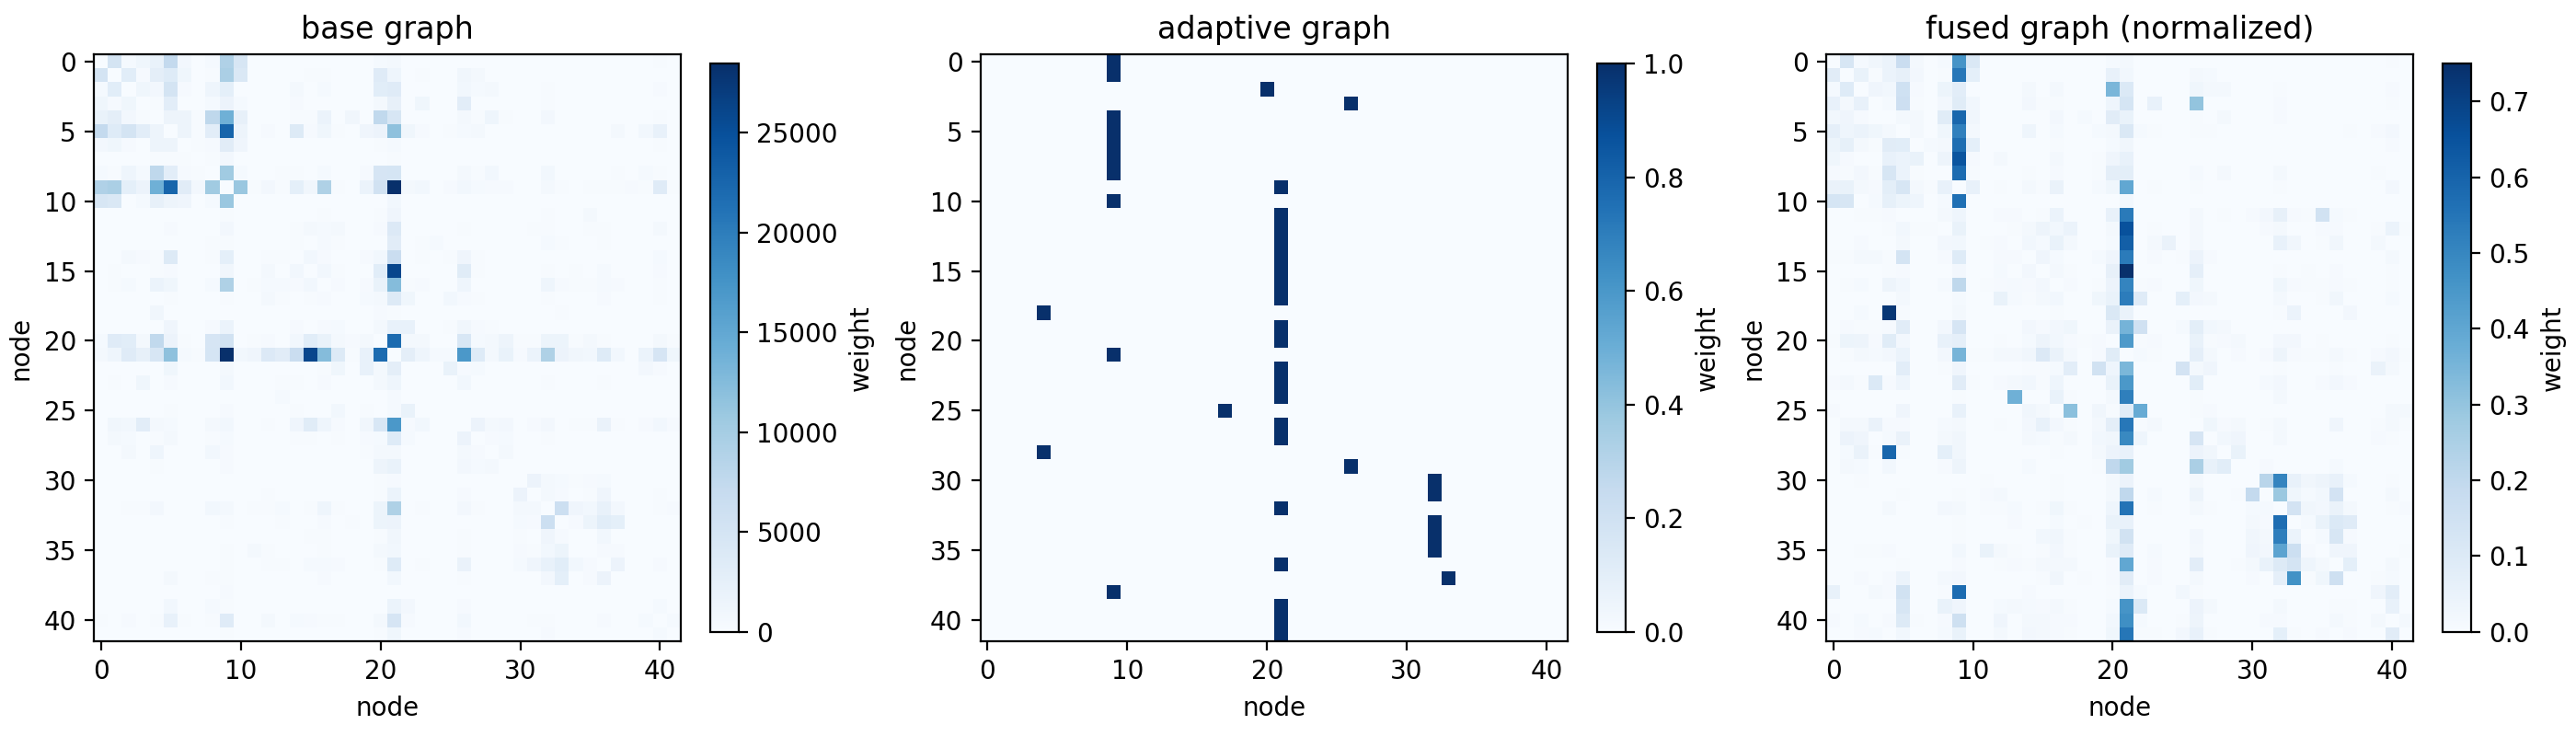
\includegraphics[height=0.095\textheight]{figs/graph_analysis_oa1/hybrid/three_graph_heatmaps.png}
        \\[-2pt]
        {\small (a) \texttt{domain 1}: base $\rightarrow$ adaptive $\rightarrow$ fused}
        \vspace{6pt}

        
\includegraphics[height=0.095\textheight]{figs/graph_analysis_oa1702/hybrid/three_graph_heatmaps.png}
        \\[-2pt]
        {\small (b) \texttt{subfield 1702}: base $\rightarrow$ adaptive $\rightarrow$ fused}
    \end{minipage}\hfill
    \begin{minipage}[t]{0.40\linewidth}
        \centering
        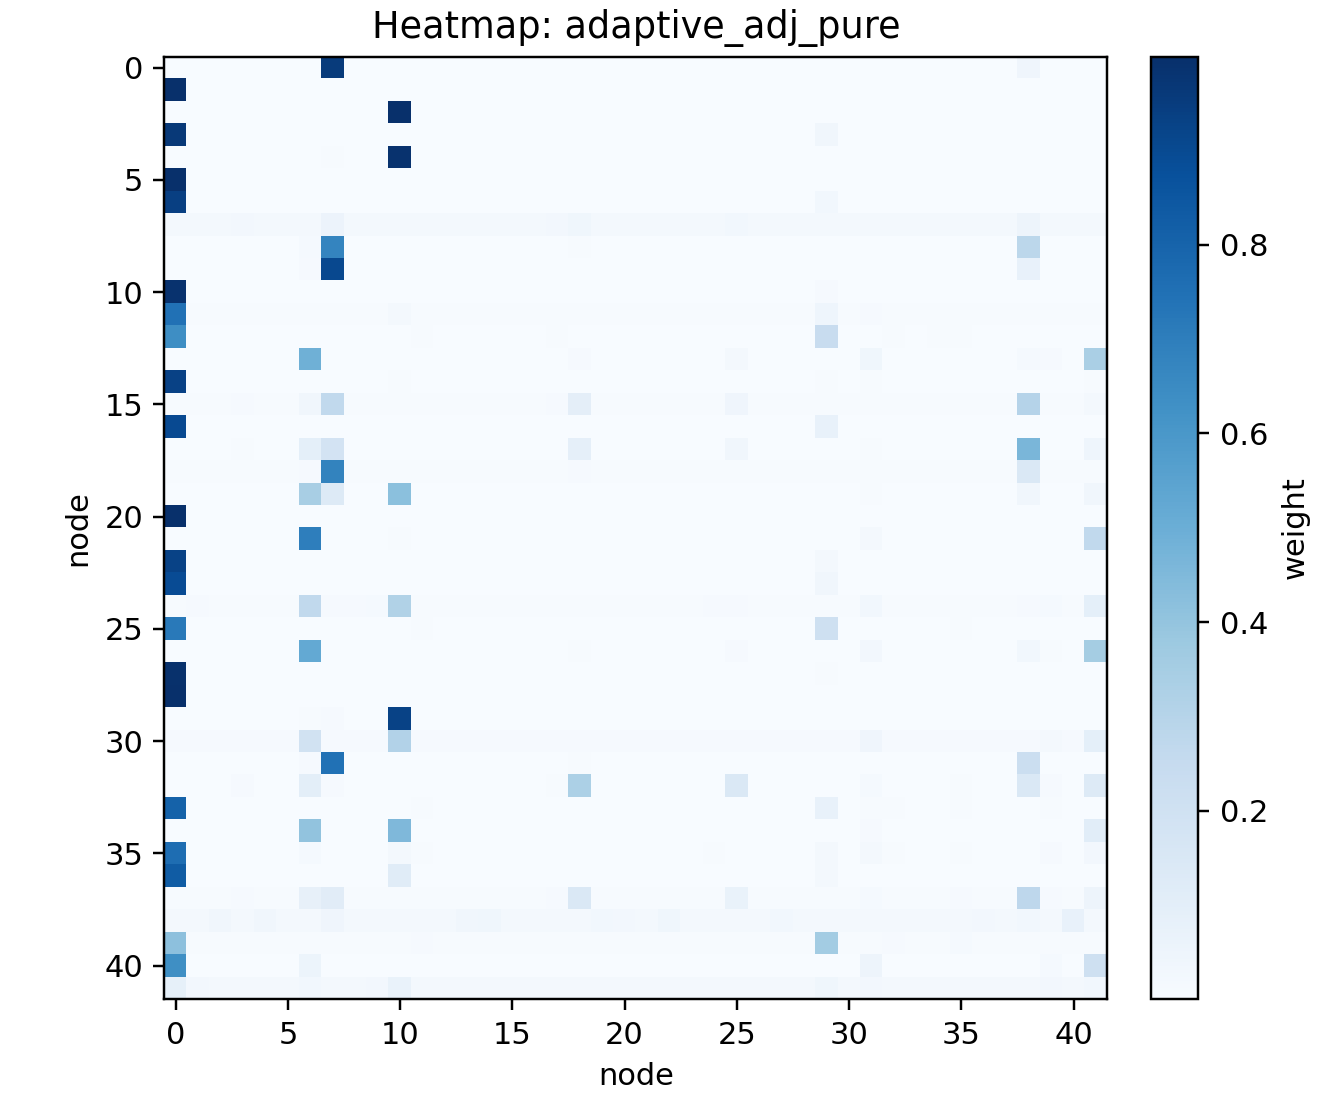
\includegraphics[height=0.095\textheight]{figs/graph_analysis_oa1/adaptive_only/adaptiveonly_adaptivegraph_heatmap.png}
        \\[-2pt]
        {\small (c) \texttt{domain 1}: adaptive-only}
        \vspace{6pt}

        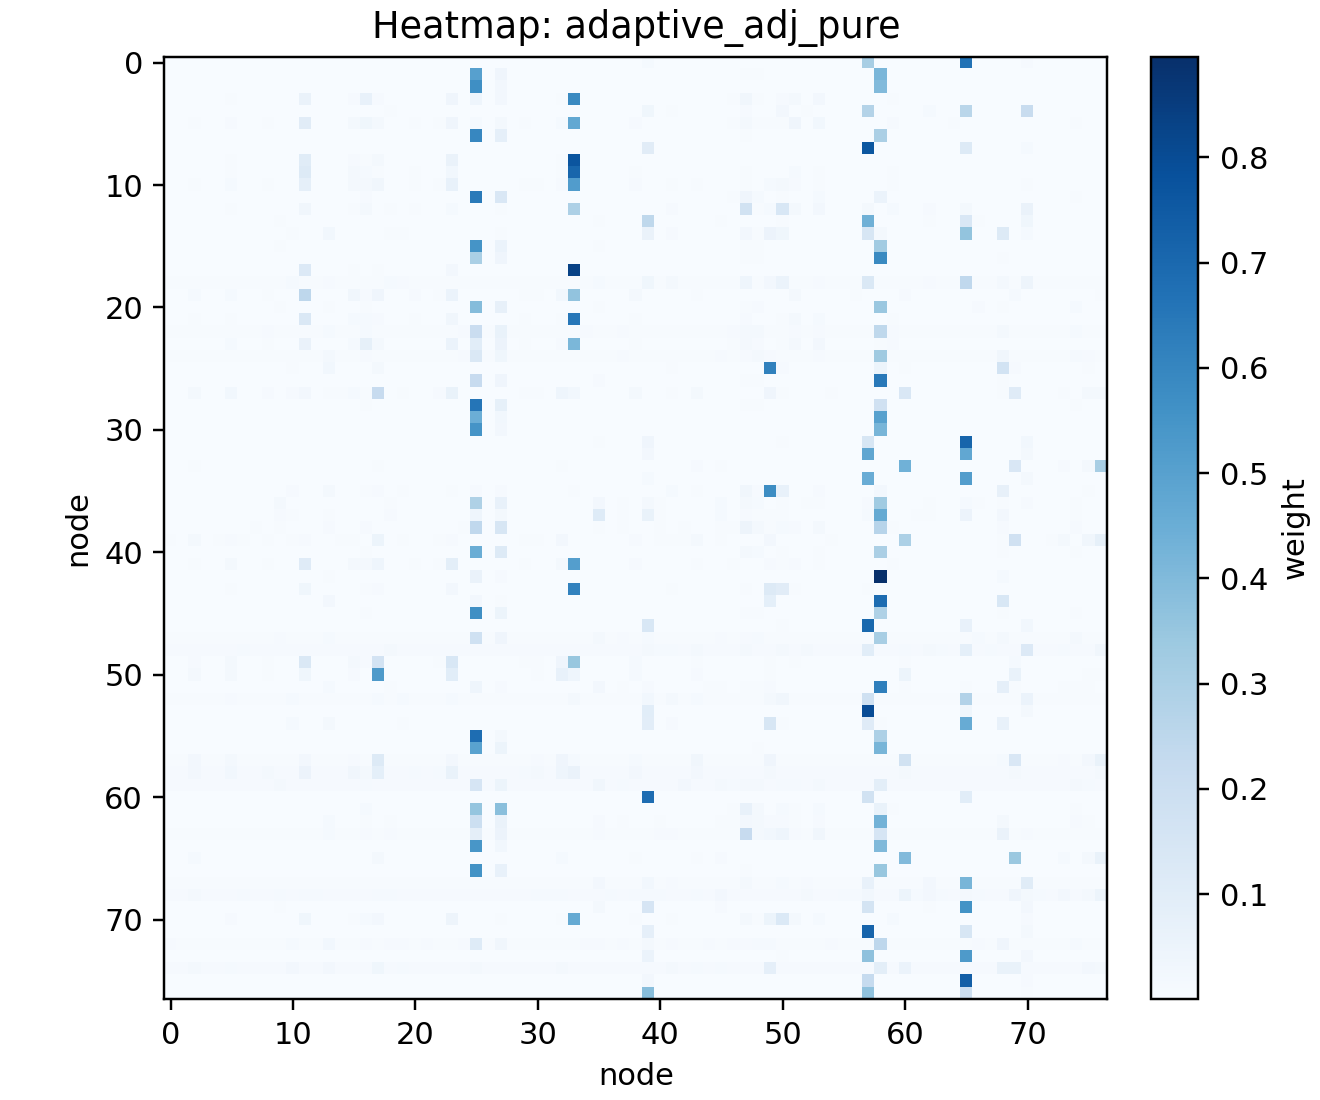
\includegraphics[height=0.095\textheight]{figs/graph_analysis_oa1702/adaptive_only/adaptiveonly_adaptivegraph__heatmap.png}
        \\[-2pt]
        {\small (d) \texttt{subfield 1702}: adaptive-only}
    \end{minipage}
    \caption{Topology comparison overview. Left: matrix-level transition (base $\rightarrow$ adaptive $\rightarrow$ fused). Right: adaptive-only heatmaps.}
    \label{fig:relation-merged}
\end{figure}

Figure~\ref{fig:relation-merged} provides global evidence of topology transition from prior co-occurrences to learned and fused relations. Consistent with the main-text exploratory analysis, domain-level and subfield-level subsets start from different sparsity regimes, which directly affects fusion behavior. For \texttt{domain 1}, where the prior graph is already dense (1,440 off-diagonal edges, 83.62\%), fusion mainly performs directional reweighting over existing support. For \texttt{subfield 1702}, where the prior graph is sparser (2,254 edges, 38.52\%), fusion becomes denser (2,979 edges, 50.91\%), indicating stronger supplementation beyond raw co-occurrence.

\begin{table}[htbp]
    \caption[Representative potential relationships from hybrid topology.]{Representative potential relationships from hybrid topology.}
    \label{tab:relation-cases}
    \centering
    \begingroup
    \scriptsize
    \setlength{\tabcolsep}{3pt}
    \renewcommand{\arraystretch}{1.10}
    \resizebox{\textwidth}{!}{%
    \begin{tabular}{>{\centering\arraybackslash}m{0.14\textwidth}>{\raggedright\arraybackslash}m{0.36\textwidth}>{\centering\arraybackslash}m{0.09\textwidth}>{\centering\arraybackslash}m{0.09\textwidth}>{\centering\arraybackslash}m{0.09\textwidth}>{\raggedright\arraybackslash}m{0.17\textwidth}}
        \toprule
        Level & Relation (source $\rightarrow$ target) & Base (rel.) & Adaptive & Fused & Observation \\
        \midrule
        domain 1 & Cancer Research (1306) $\rightarrow$ Molecular Biology (1312) & 0.9104 & 1.0000 & 0.7499 & Prior-consistent and strongly promoted \\
        domain 1 & Molecular Biology (1312) $\rightarrow$ Cancer Research (1306) & 0.9104 & 0.0000 & 0.1013 & Same prior pair but suppressed reverse direction \\
        domain 1 & Horticulture (1108) $\rightarrow$ Plant Science (1110) & 0.0262 & 1.0000 & 0.6432 & Prior edge kept and direction sharpened \\
        \midrule
        subfield 1702 & Quantum Information and Cryptography (10020) $\rightarrow$ Quantum Computing Algorithms and Architecture (10682) & 0.5403 & 1.0000 & 0.8741 & Strong prior link retained after fusion \\
        subfield 1702 & Semantic Web and Ontologies (10215) $\rightarrow$ Natural Language Processing Techniques (10181) & 0.0452 & 1.0000 & 0.6361 & Directed refinement from symmetric co-occurrence \\
        subfield 1702 & Experience-Based Knowledge Management (13514) $\rightarrow$ Multi-Agent Systems and Negotiation (10456) & 0.0000 & 0.9998 & 0.8390 & Newly discovered latent relation \\
	    \bottomrule
		    \end{tabular}%
		    }
		    \endgroup
\vspace{2pt}
{\raggedright\footnotesize\textit{Note:} Base (rel.) is normalized within each subset by the maximum off-diagonal base-edge weight (domain 1: 28,443; subfield 1702: 9,294).\par}
\end{table}

Table~\ref{tab:relation-cases} highlights representative links. In \texttt{domain 1}, links such as Cancer Research $\rightarrow$ Molecular Biology demonstrate a calibration effect, where prior-supported edges are preserved but refined in strength and direction. In \texttt{subfield 1702}, the topology preserves strong priors while activating newly discovered relations, such as Experience-Based Knowledge Management $\rightarrow$ Multi-Agent Systems and Negotiation.

Quantitatively, \texttt{hybrid} and \texttt{adaptive only} exhibit distinct behaviors. At equal edge budget, \texttt{hybrid} maintains much higher prior overlap (100\% vs.\ 82.3\% on \texttt{domain 1}; 92.0\% vs.\ 36.6\% on \texttt{subfield 1702}) and more diversified top-1 targets. By contrast, \texttt{adaptive only} is more hub-concentrated, matching the dark-column pattern in Fig.~\ref{fig:relation-merged}(c,d); for example, 42 nodes in \texttt{domain 1} collapse to 7 top-1 targets.

These topologies reveal structured associations but do not, by themselves, establish causal mechanisms behind forecast improvements. Robust attribution requires dedicated explanatory tests, such as dynamic link validation against future co-occurrence evolution, Granger-style temporal causality analysis, or perturbation-based edge-level interventions (e.g., SHAP).

Overall, \texttt{adaptive only} is preferable when pure predictive fitting is the main objective, whereas \texttt{hybrid} is preferable when downstream scientometric analysis requires prior-grounded relation evidence.

\subsection{Five-Year Trajectory Forecasts of Representative Topics}
\label{sec:appendix-hotspots}
Figure~\ref{fig:trend-pair} presents five-year forecasts (2025--2029) for representative topics in \texttt{domain 1} and \texttt{subfield 1702}. We use these trajectories to characterize potential hotspot evolution under different granularity levels. In \texttt{domain 1}, the trajectories are relatively stable and mixed: only two topics keep increasing, i.e., Food Science (\texttt{1106}, 8.59\%) and Ecology, Evolution, Behavior and Systematics (\texttt{1105}, 1.67\%). The other four topics show mild declines, including Plant Science (\texttt{1110}), Genetics (\texttt{1311}), Molecular Biology (\texttt{1312}), and Immunology (\texttt{2403}), with changes ranging from -0.53\% to -4.05\%. At the aggregate level, \texttt{domain 1} is nearly flat, changing from 892,324 in 2025 to 890,273 in 2029 (-0.23\%), which suggests a mature and saturated macro-domain pattern.

By contrast, \texttt{subfield 1702} shows stronger growth and higher divergence across topics. The total predicted volume increases from 71,315 in 2025 to 95,200 in 2029 (33.49\%). The largest acceleration appears in Educational Technology Systems (\texttt{13559}, 72.98\%), followed by Geochemistry and Geologic Mapping (\texttt{12157}, 30.08\%) and Semantic Web and Ontologies (\texttt{10215}, 23.31\%); Natural Language Processing Techniques (\texttt{10181}) and Neural Networks and Applications (\texttt{10320}) also maintain positive growth. In contrast, Advanced Computational Techniques and Applications (\texttt{13734}) declines by 6.17\%. These results indicate that, compared with the broad-domain setting, subfield-level dynamics remain more active and heterogeneous, and therefore provide clearer signals for identifying candidate future hotspot topics.

\begin{figure}[htbp]
    \centering
    \begin{minipage}[t]{0.48\linewidth}
        \centering
        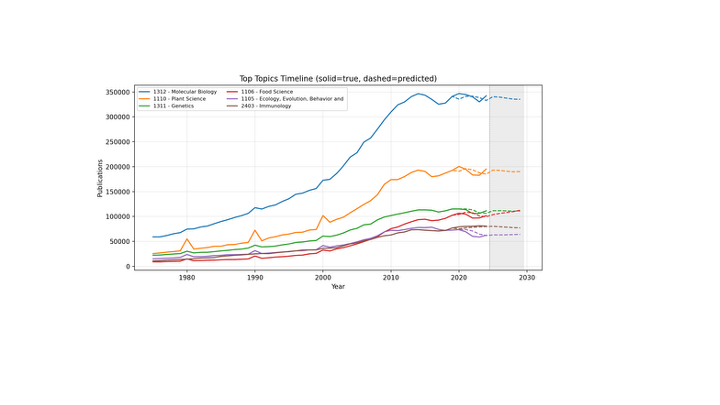
\includegraphics[width=\linewidth,trim=80 95 160 65,clip]{figs/Forecast trend visualization for oa1.png}
        \\[-2pt]
        {\small (a) Forecast trend for \texttt{domain 1}}
    \end{minipage}\hfill
    \begin{minipage}[t]{0.48\linewidth}
        \centering
        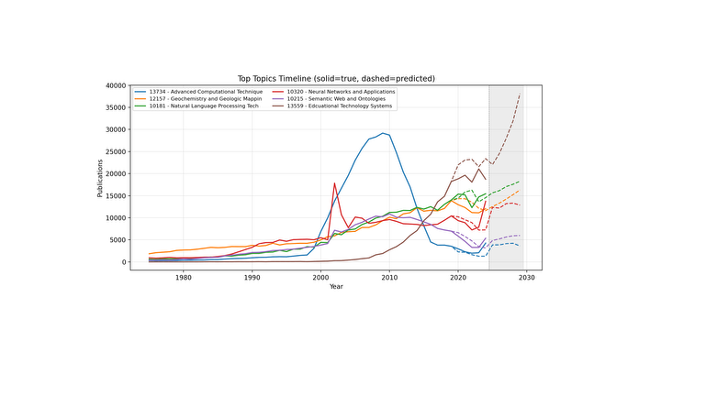
\includegraphics[width=\linewidth,trim=80 95 160 65,clip]{figs/Forecast trend visualization for oa1702.png}
        \\[-2pt]
        {\small (b) Forecast trend for \texttt{subfield 1702}}
    \end{minipage}
    \caption{Forecast trend visualizations.}
    \label{fig:trend-pair}
\end{figure}
\FloatBarrier

\subsection{Dataset Statistics and Granularity-Specific Exploratory Analysis}
\label{sec:appendix-exploratory}
\label{sec:appendix-dataset-summary}
\label{sec:appendix-pattern-diagnostics}
Table~\ref{tab:dataset-summary} reports raw-data statistics for the eight benchmark subsets, including node scale, growth profile, sparsity, and graph dynamics.

\begin{table}[htbp]
\caption[Dataset summary and raw-data statistics of the eight benchmark subsets.]{Dataset summary and raw-data statistics of the eight benchmark subsets.}
\label{tab:dataset-summary}
\centering
\begingroup
\scriptsize
\setlength{\tabcolsep}{2.6pt}
\renewcommand{\arraystretch}{1.12}
\resizebox{\textwidth}{!}{%
\begin{tabular}{>{\centering\arraybackslash}m{2.35cm}>{\centering\arraybackslash}m{1.45cm}c c >{\raggedright\arraybackslash}m{3.20cm}c c c c c c c}
\toprule
Subset & Prediction target & $N$ & Example ID & Example description & Years & \shortstack[c]{Total vol.\\(start)} & \shortstack[c]{Total vol.\\(end)} & Growth ratio & \shortstack[c]{Zero-entry\\ratio} & \shortstack[c]{Avg. graph\\density} & \shortstack[c]{Avg. edge\\turnover} \\
\midrule
domain 1 (Life Sciences) & subfield popularity & 42 & 1100 & plant and animal cultivation for useful products & 1975--2024 & 258312 & 1644473 & 6.37 & 0.05\% & 75.79\% & 10.32\% \\
domain 2 (Social Sciences) & subfield popularity & 58 & 1200 & study of human culture, including art and artifacts & 1975--2024 & 279427 & 3288467 & 11.77 & 0.00\% & 84.24\% & 8.66\% \\
domain 3 (Physical Sciences) & subfield popularity & 89 & 1502 & bioengineering for practical product development & 1975--2024 & 601096 & 5139713 & 8.55 & 0.00\% & 73.92\% & 11.47\% \\
domain 4 (Health Sciences) & subfield popularity & 63 & 2702 & anatomy: structure and parts of organisms & 1975--2024 & 350998 & 3082956 & 8.78 & 0.00\% & 80.95\% & 8.76\% \\
subfield 1702 (Artificial Intelligence) & topic popularity & 77 & 12761 & concept-drift adaptation in streaming machine learning & 1975--2024 & 12803 & 346565 & 27.07 & 0.31\% & 22.05\% & 36.46\% \\
subfield 1705 (Computer Networks and Communications) & topic popularity & 43 & 10249 & distributed multi-agent coordination and consensus control & 1975--2024 & 6612 & 135497 & 20.49 & 0.98\% & 34.78\% & 28.56\% \\
subfield 1707 (Computer Vision and Pattern Recognition) & topic popularity & 35 & 10036 & deep-learning methods for vision recognition tasks & 1975--2024 & 3766 & 182490 & 48.46 & 0.29\% & 49.31\% & 28.90\% \\
subfield 1710 (Information Systems) & topic popularity & 78 & 10679 & QoS-aware web-service composition and semantic matching & 1975--2024 & 4904 & 297164 & 60.60 & 0.92\% & 14.87\% & 45.58\% \\
\bottomrule
\end{tabular}%
}
\endgroup
\vspace{2pt}
{\raggedright\footnotesize\textit{Note:} Definitions: \textit{Total vol.} is annual summed node volume; \textit{Growth ratio} is the end-to-start ratio; \textit{Zero-entry ratio} is the share of zero year-node entries; \textit{Avg. graph density} is mean yearly co-occurrence density; \textit{Avg. edge turnover} is mean year-to-year edge-set Jaccard change.\par}
\end{table}

Complementing this tabular summary, Figure~\ref{fig:dataset-pair} visualizes two representative subsets with different granularity: \texttt{domain 1} (domain-level) and \texttt{subfield 1702} (subfield-level). Each subset in this figure contains 30 topics with annual observations from 1975 to 2024.

\begin{figure}[htbp]
    \centering
    \begin{minipage}[t]{0.485\linewidth}
        \centering
        \begin{minipage}[t]{0.43\linewidth}
            \centering
            \vspace{0pt}
            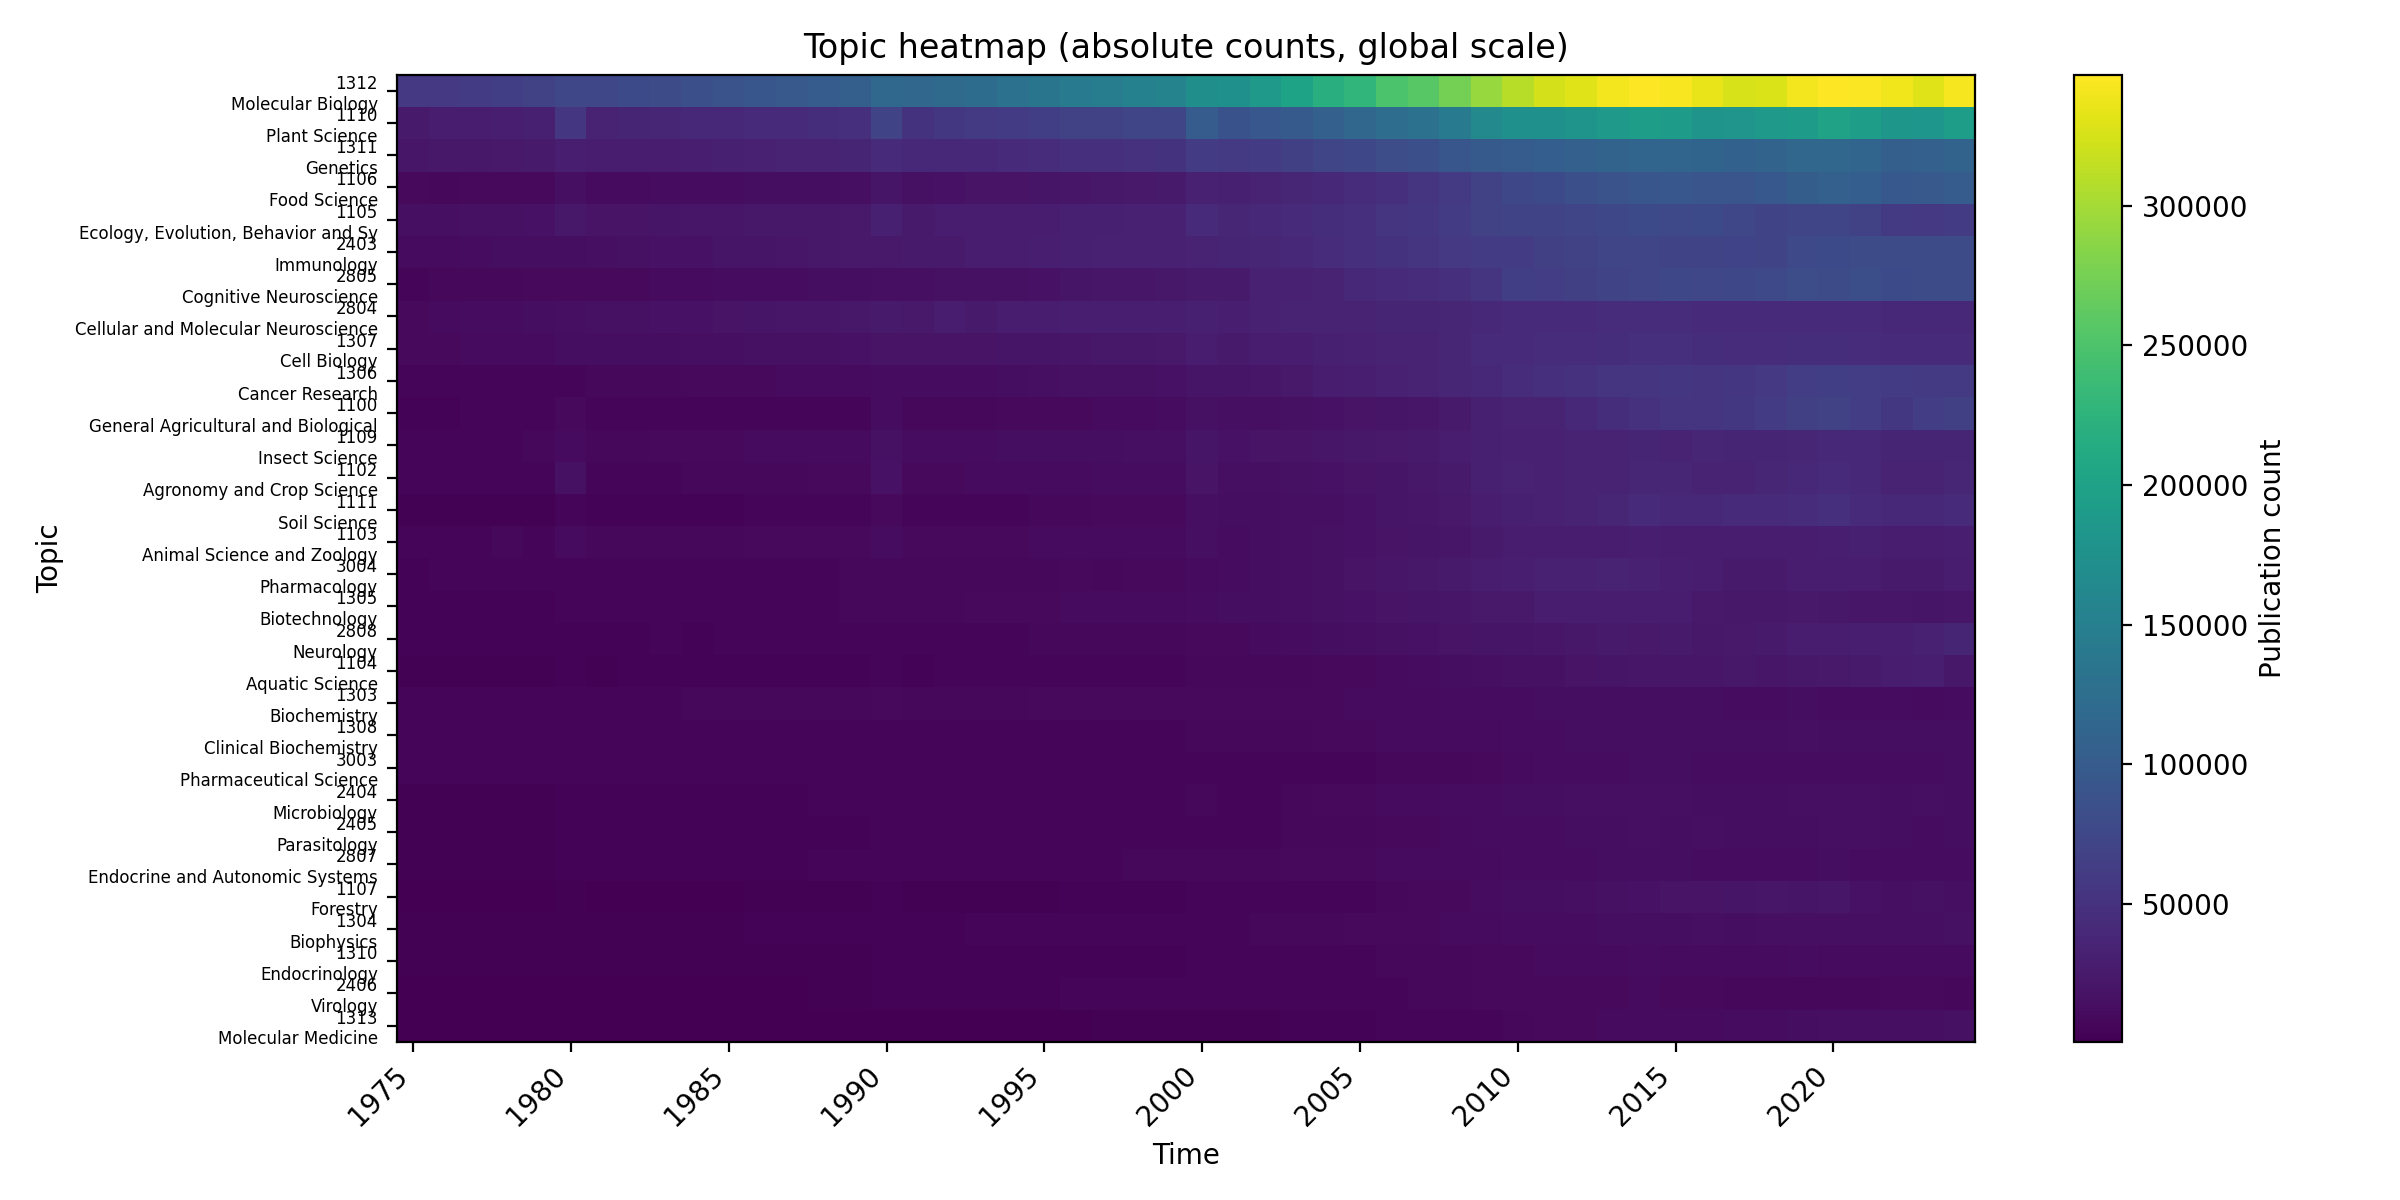
\includegraphics[height=0.070\textheight,keepaspectratio]{figs/data_analysis/oa_1_heatmap_all.png}
            \par\vspace{1pt}
            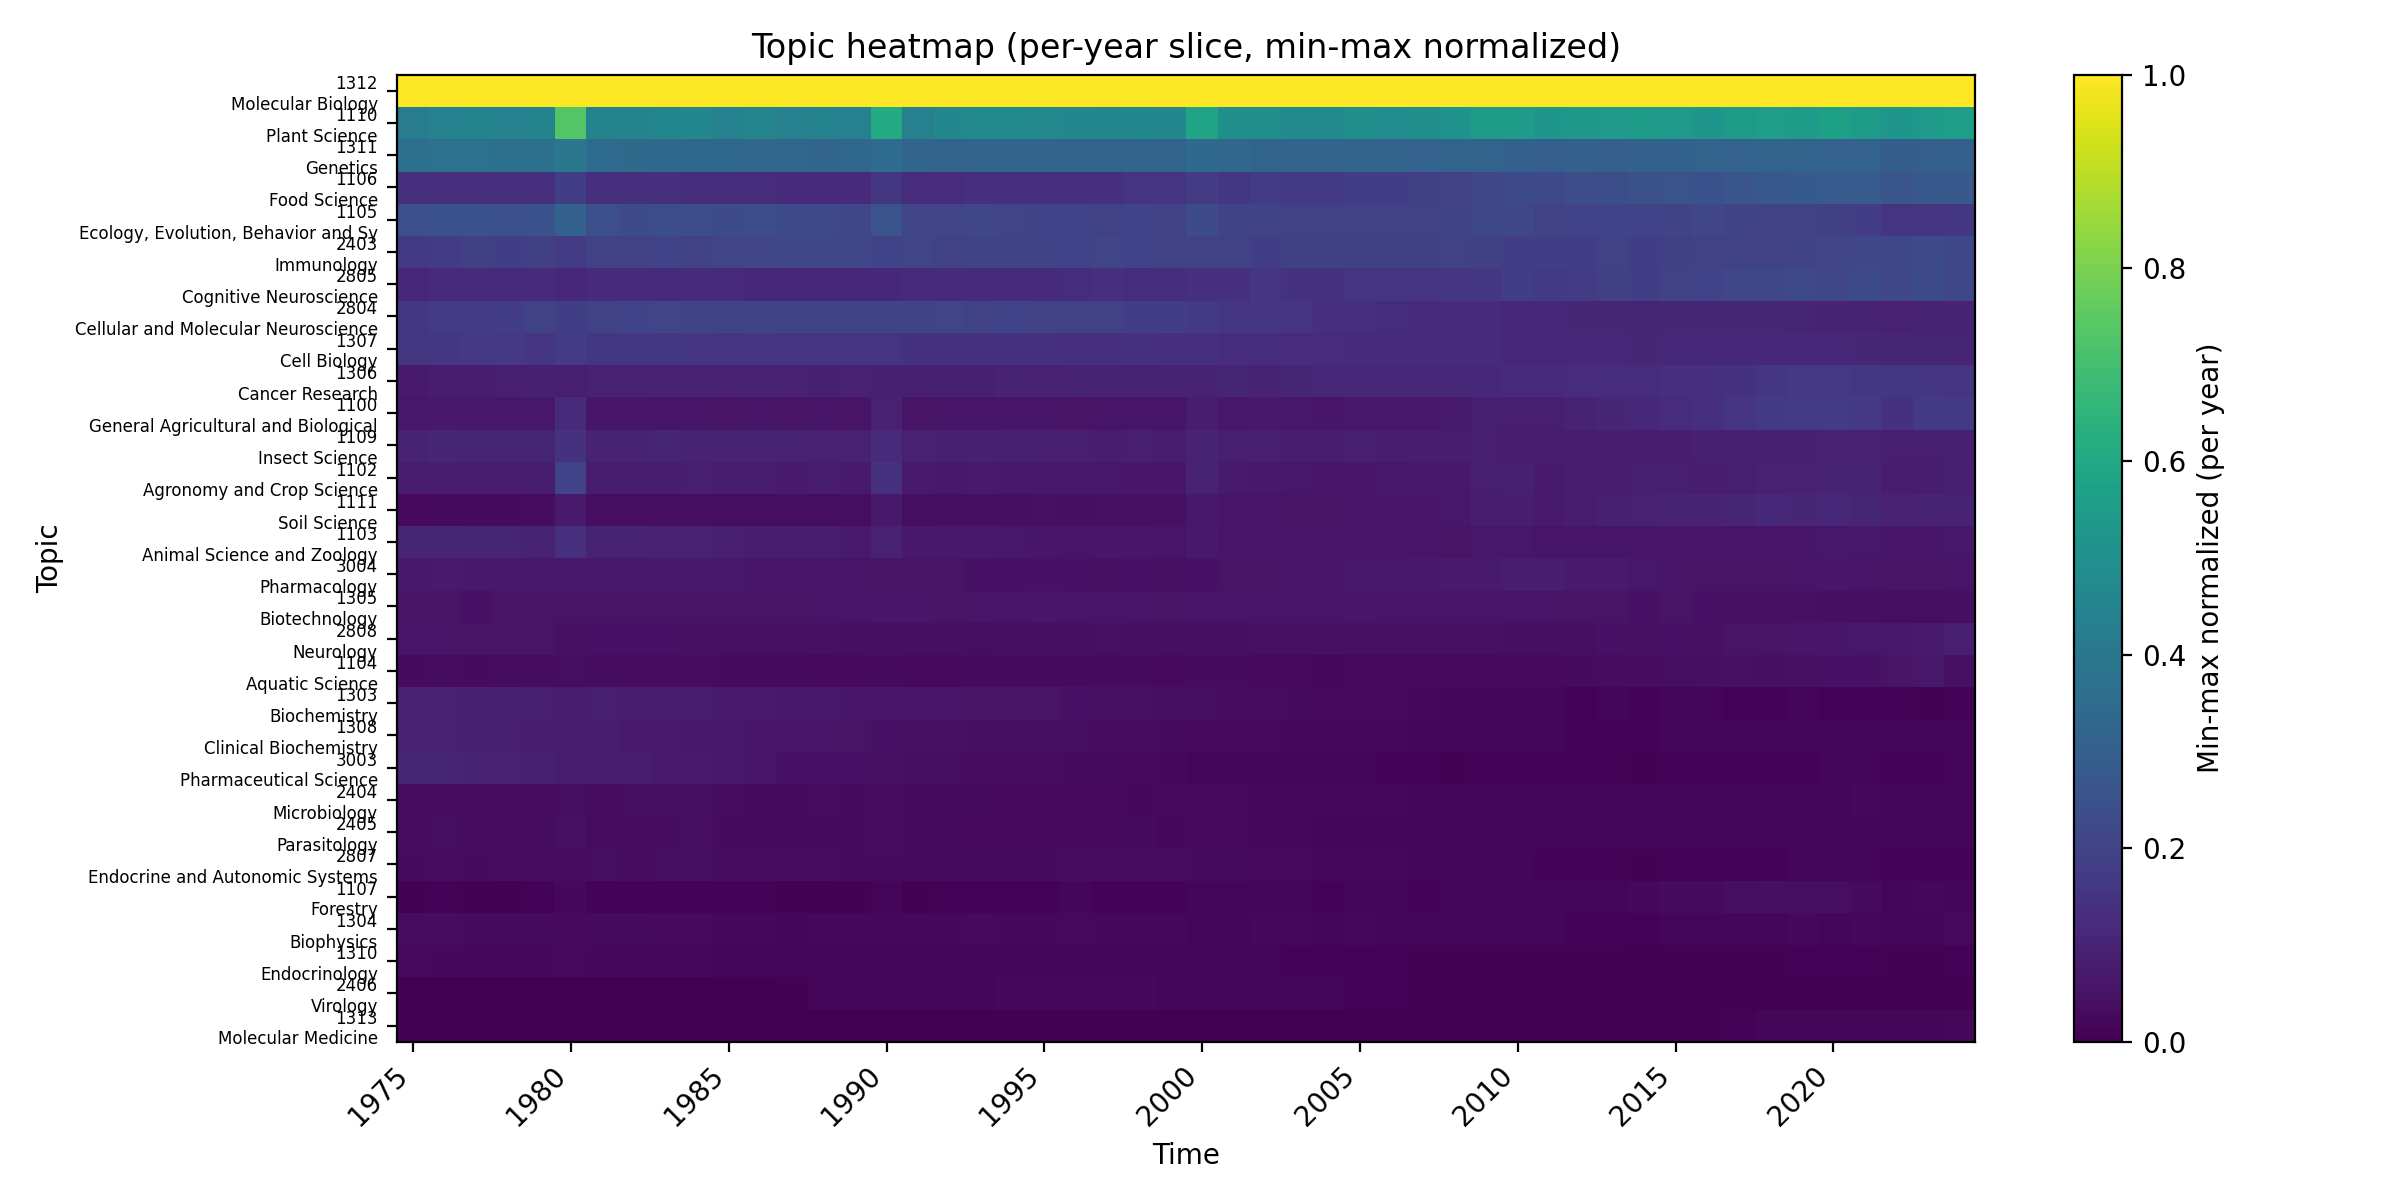
\includegraphics[height=0.070\textheight,keepaspectratio]{figs/data_analysis/oa_1_heatmap_year_minmax.png}
            \par\vspace{1pt}
            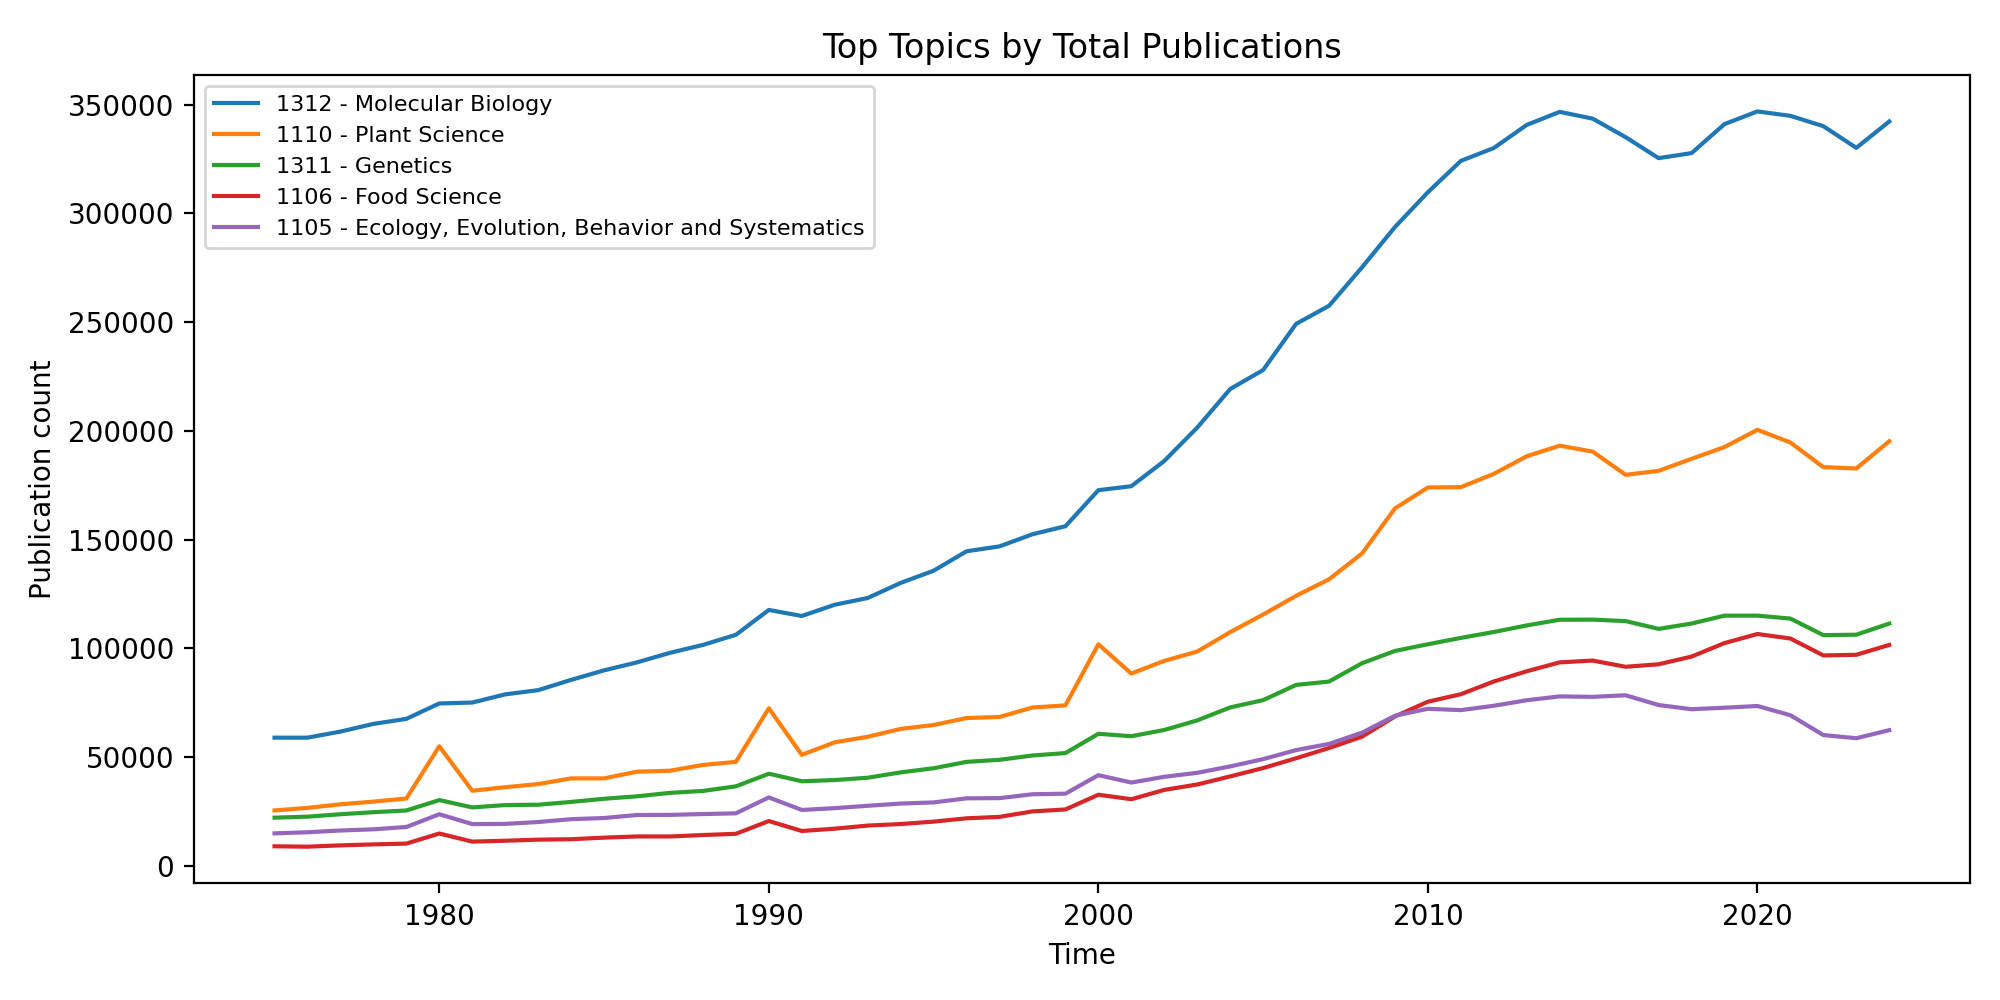
\includegraphics[height=0.070\textheight,keepaspectratio]{figs/data_analysis/oa_1_top_topics.png}
        \end{minipage}\hfill
        \begin{minipage}[t]{0.53\linewidth}
            \centering
            \vspace{0pt}
            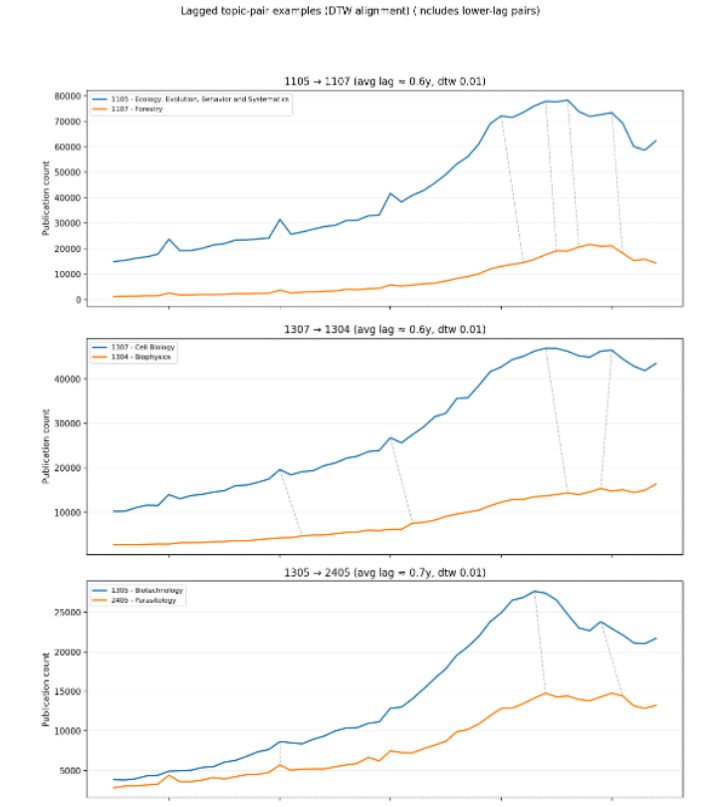
\includegraphics[height=0.220\textheight,keepaspectratio]{figs/data_analysis/DTW_oa1.png}
        \end{minipage}
        \par\vspace{1pt}
        {\small \textbf{(a) \texttt{domain 1}}}
    \end{minipage}\hfill
    \begin{minipage}[t]{0.485\linewidth}
        \centering
        \begin{minipage}[t]{0.43\linewidth}
            \centering
            \vspace{0pt}
            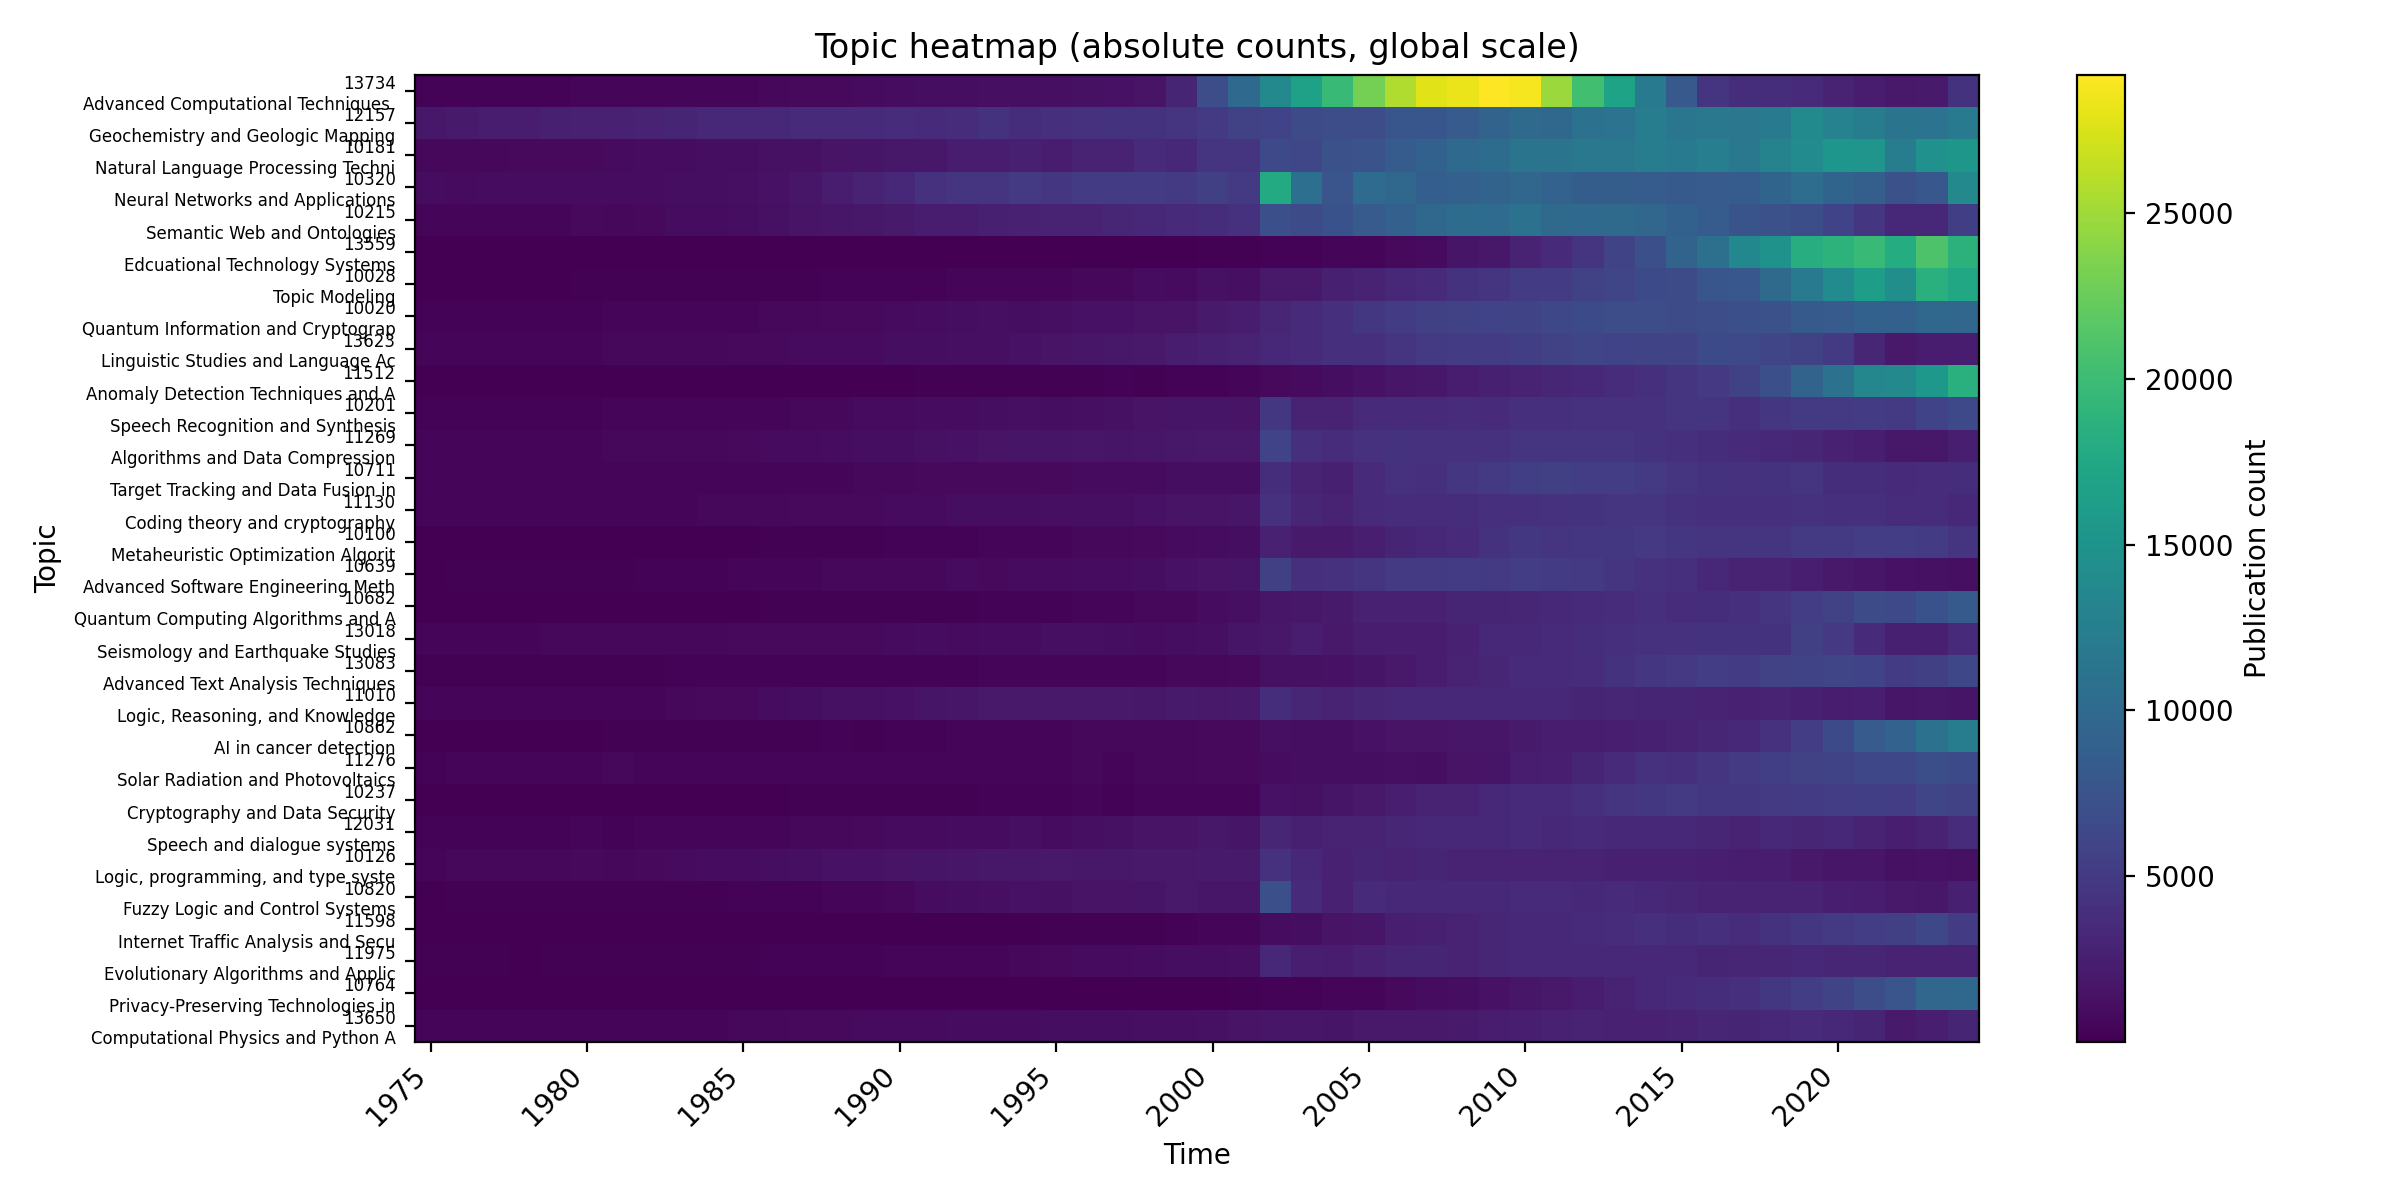
\includegraphics[height=0.070\textheight,keepaspectratio]{figs/data_analysis/oa_1702_heatmap_all.png}
            \par\vspace{1pt}
            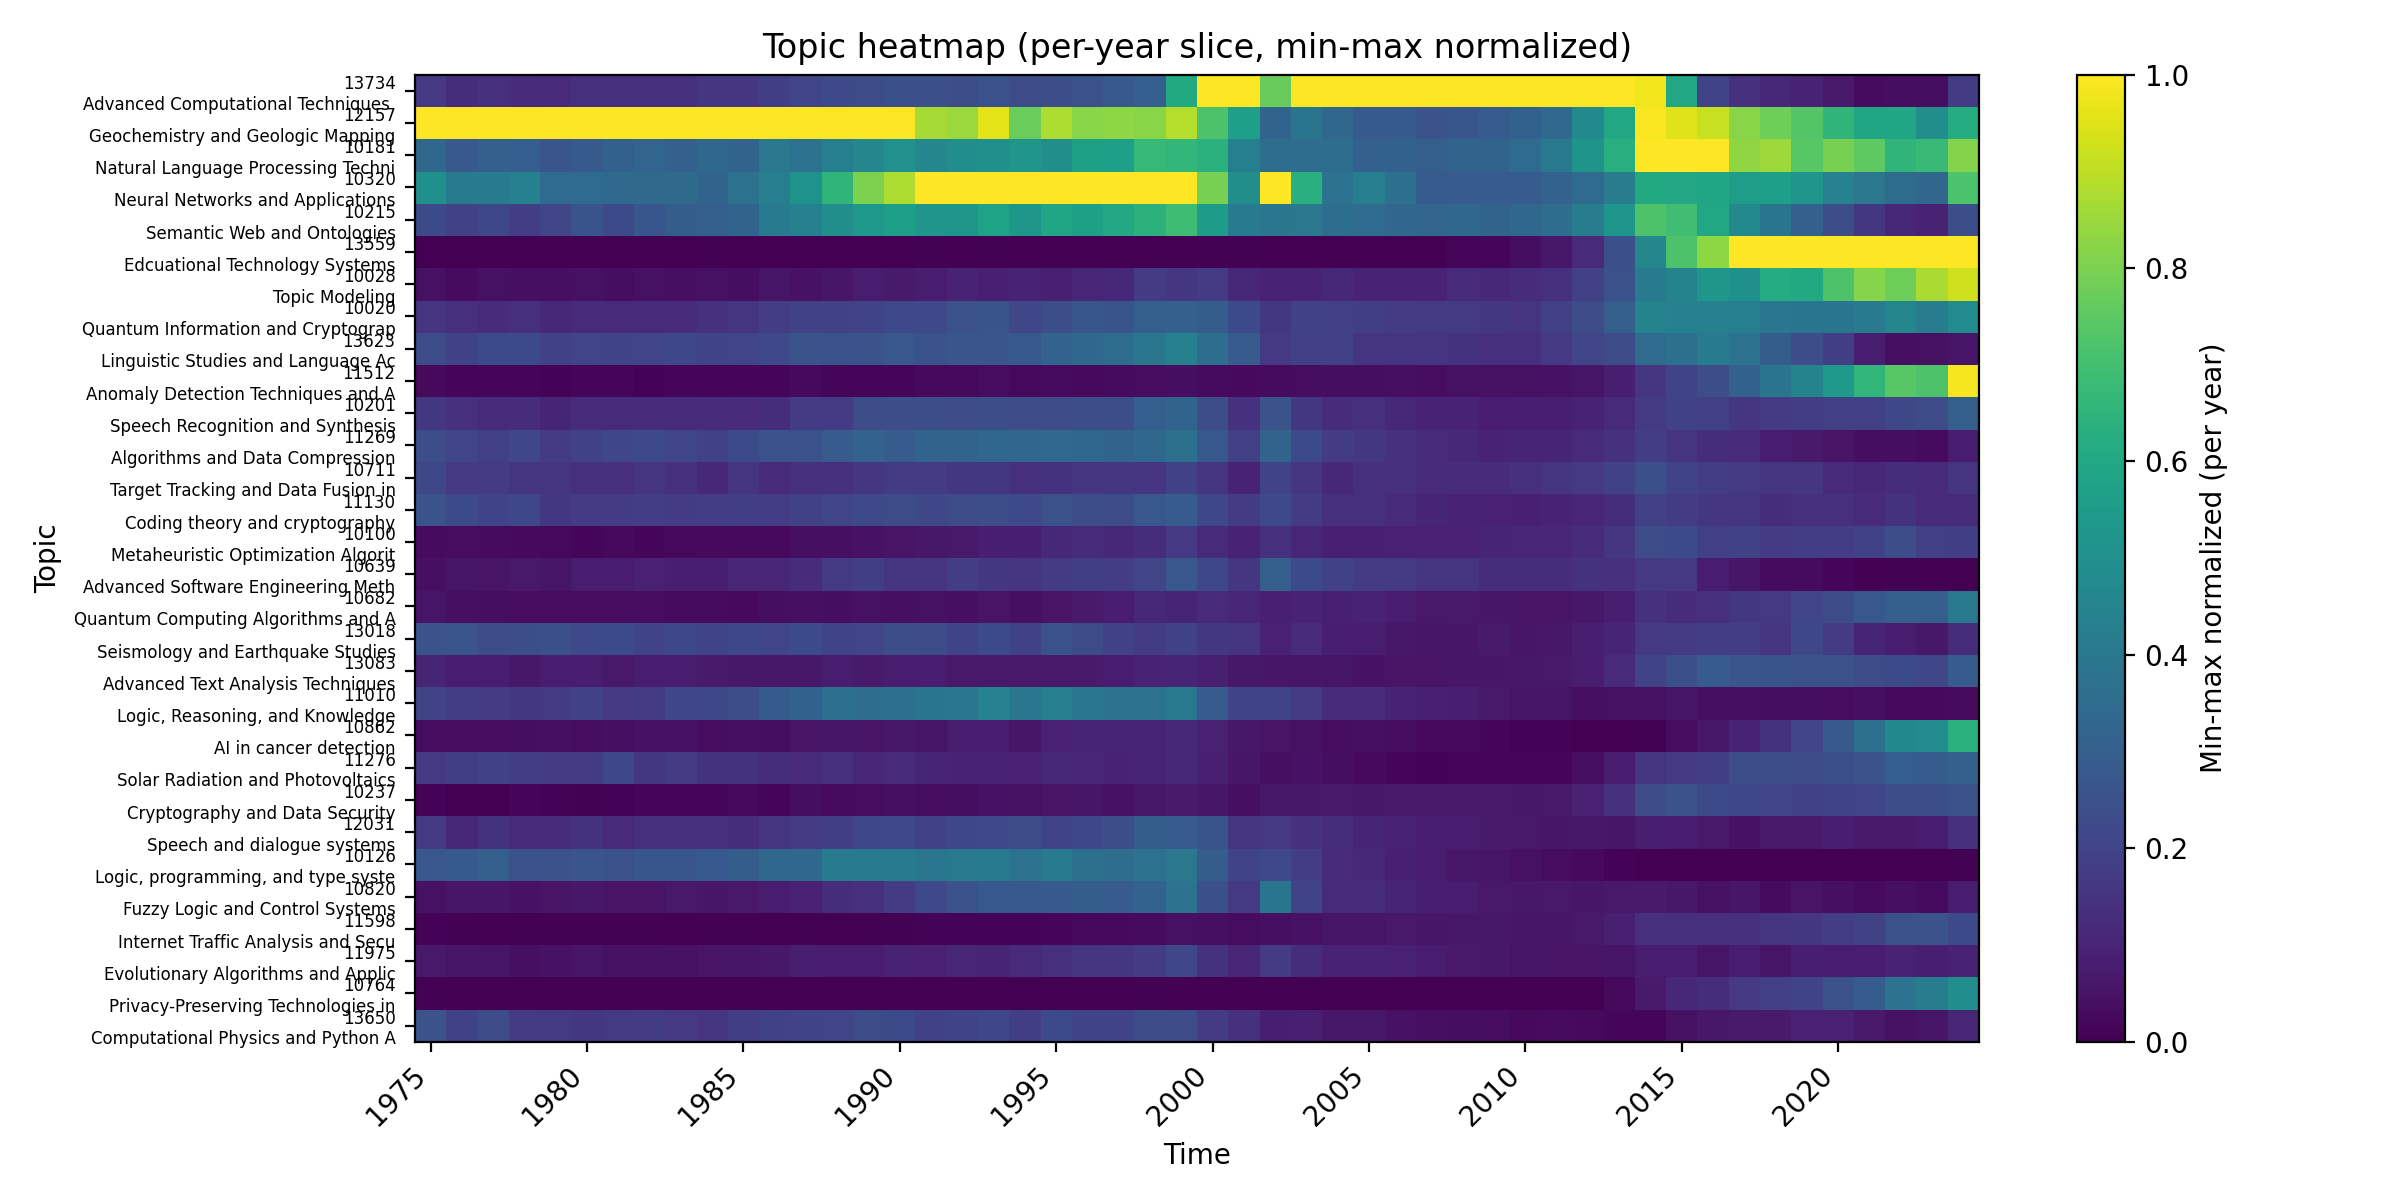
\includegraphics[height=0.070\textheight,keepaspectratio]{figs/data_analysis/oa_1702_heatmap_year_minmax.png}
            \par\vspace{1pt}
            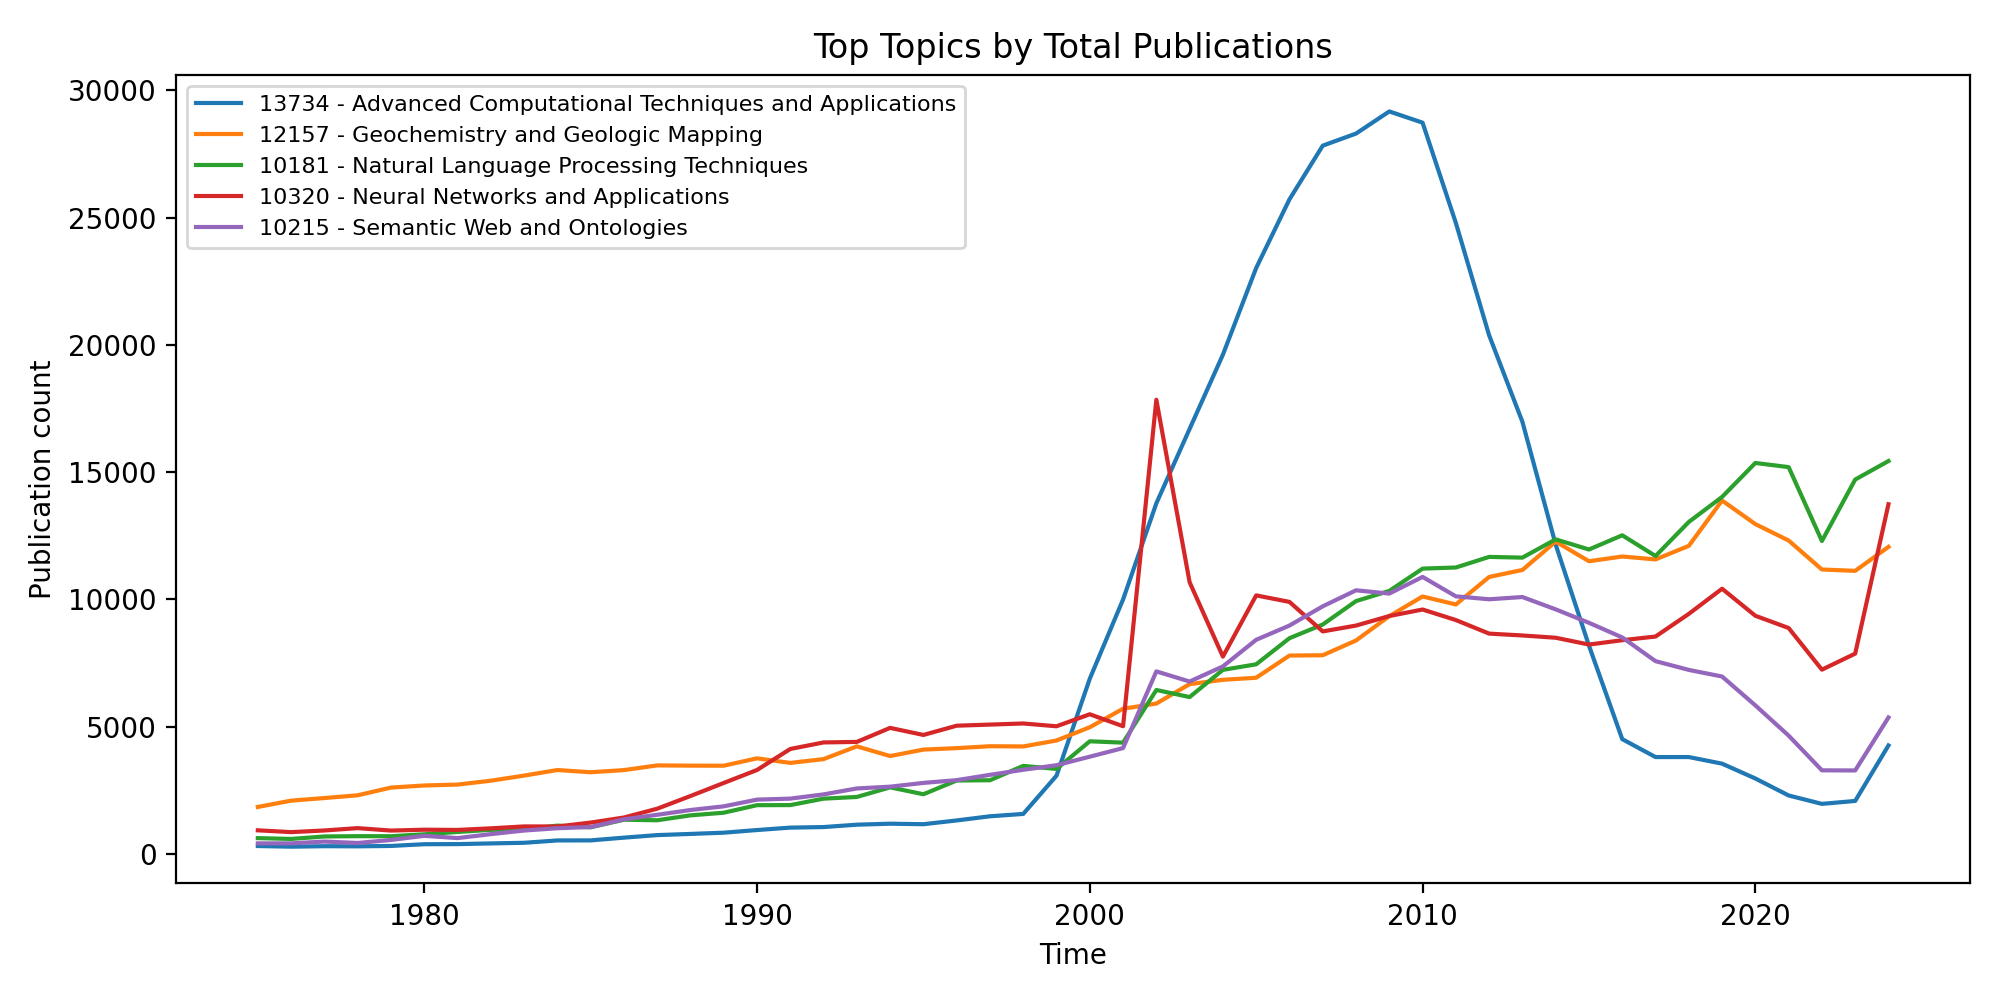
\includegraphics[height=0.070\textheight,keepaspectratio]{figs/data_analysis/oa_1702_top_topics.png}
        \end{minipage}\hfill
        \begin{minipage}[t]{0.53\linewidth}
            \centering
            \vspace{0pt}
            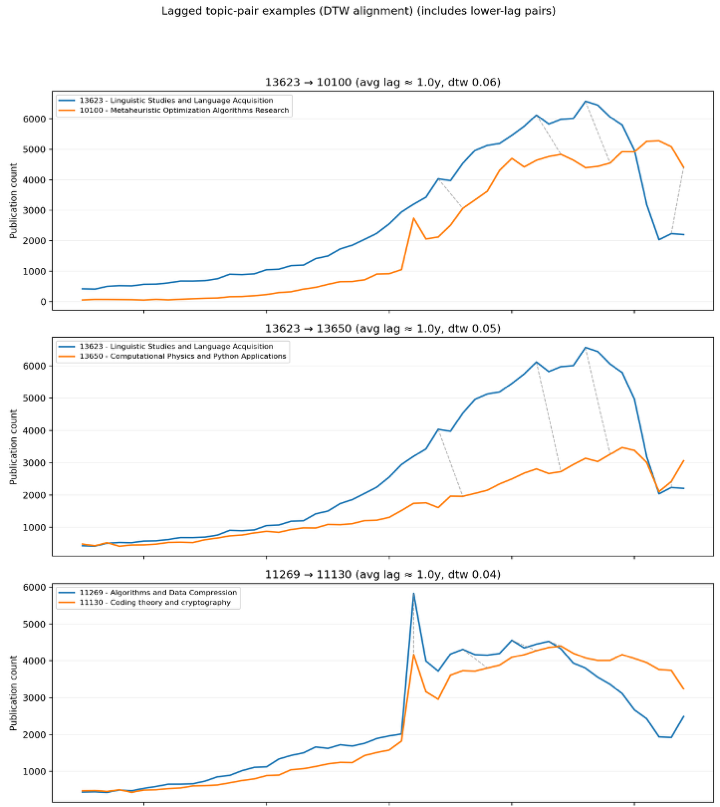
\includegraphics[height=0.220\textheight,keepaspectratio]{figs/data_analysis/DTW_oa1702.png}
        \end{minipage}
        \par\vspace{1pt}
        {\small \textbf{(b) \texttt{subfield 1702}}}
    \end{minipage}

    \caption{Dataset pattern illustrations for \texttt{domain 1} and \texttt{subfield 1702}. In each dataset block, the left column vertically stacks \texttt{heatmap\_all}, \texttt{heatmap\_year\_minmax}, and \texttt{top\_topics}, while the right column shows \texttt{DTW}.}
    \label{fig:dataset-pair}
\end{figure}
\FloatBarrier

For \texttt{domain 1}, the absolute-count heatmap and top-topic curves show steady long-term growth with a relatively stable hierarchy. The total publication volume increases from 249,648 to 1,582,343 (533.8\%). At the same time, concentration remains high but stable: the top-1 topic share changes from 23.60\% to 21.63\%, and the top-5 share stays near 53\% (52.92\% to 52.53\%). The leading topics (e.g., Molecular Biology, Plant Science, and Genetics) mostly peak around 2020, indicating persistent head-topic dominance with gradual diffusion to other topics.

For \texttt{subfield 1702}, the same analyses reveal faster expansion but stronger structural turnover. Total volume grows from 9,856 to 211,684 (2047.8\%), while concentration drops more clearly: top-1 share decreases from 18.73\% to 8.84\%, and top-5 share from 44.40\% to 39.61\%. Topic peaks are asynchronous (e.g., Neural Networks and Applications peaks in 2002, Advanced Computational Techniques and Applications in 2009, Semantic Web and Ontologies in 2010, and NLP-related topics continue rising to 2024), which is consistent with the higher year-wise dispersion in the min-max heatmap.

DTW panels further show meaningful lagged dependencies. In \texttt{domain 1}, aligned pairs have shorter average lag (0.572 years), lower average DTW distance (0.0086), and higher average correlation (0.991), suggesting smoother co-evolution. In \texttt{subfield 1702}, pairs exhibit longer lag (0.900 years), larger DTW distance (0.0386), and lower correlation (0.965), reflecting more heterogeneous and phase-shifted dynamics.

Taken together, Figure~\ref{fig:dataset-pair} highlights two facts that are central to this task: (1) research hotspots can change quickly in some subsets, especially at the subfield level (e.g., \texttt{subfield 1702}); and (2) some topic pairs show clear lagged correlation patterns. Therefore, reliable forecasting should not rely on independent univariate series only, but should explicitly integrate graph-structured topic relations with temporal dynamics.

\end{document}
